%==============================================================================00
% Options for packages loaded elsewhere
\PassOptionsToPackage{unicode}{hyperref}
\PassOptionsToPackage{hyphens}{url}
%==============================================================================01
\documentclass[11pt, oneside, openany]{scrbook}
\setkomafont{disposition}{\bfseries}
\usepackage{mathptmx}
\usepackage{lipsum}
%==============================================================================03
% Make chapter pages have numbering at top right
\usepackage{fancyhdr}
\pagestyle{fancy}
\lhead{}
\chead{}
\rhead{\thepage}
\lfoot{}
\cfoot{}
\rfoot{}
\renewcommand{\headrulewidth}{0pt}
\makeatletter
\renewcommand\chapter{\if@openright\cleardoublepage\else\clearpage\fi
                    \thispagestyle{fancy}%
                    \global\@topnum\z@
                    \@afterindentfalse
                    \secdef\@chapter\@schapter}
\makeatother
%==============================================================================03
\usepackage{lmodern}
\usepackage{setspace}
%==============================================================================04
\usepackage{amssymb,amsmath}
%==============================================================================05
\usepackage{ifxetex,ifluatex}
\ifnum 0\ifxetex 1\fi\ifluatex 1\fi=0 % if pdftex
  \usepackage[T1]{fontenc}
  \usepackage[utf8]{inputenc}
  \usepackage{textcomp} % provide euro and other symbols
\else % if luatex or xetex
  \usepackage{unicode-math}
  \defaultfontfeatures{Scale=MatchLowercase}
  \defaultfontfeatures[\rmfamily]{Ligatures=TeX,Scale=1}
\fi
%==============================================================================06
% Use upquote if available, for straight quotes in verbatim environments
\IfFileExists{upquote.sty}{\usepackage{upquote}}{}
\IfFileExists{microtype.sty}{% use microtype if available
  \usepackage[]{microtype}
  \UseMicrotypeSet[protrusion]{basicmath} % disable protrusion for tt fonts
}{}
\makeatletter
\@ifundefined{KOMAClassName}{% if non-KOMA class
  \IfFileExists{parskip.sty}{%
    \usepackage{parskip}
  }{% else
    \setlength{\parindent}{0pt}
    \setlength{\parskip}{6pt plus 2pt minus 1pt}}
}{% if KOMA class
  \KOMAoptions{parskip=half}}
\makeatother
%==============================================================================07
\usepackage[table]{xcolor}
%==============================================================================08
\IfFileExists{xurl.sty}{\usepackage{xurl}}{} % add URL line breaks if available
\IfFileExists{bookmark.sty}{\usepackage{bookmark}}{\usepackage{hyperref}}
\hypersetup{
  pdftitle={Application of a Principaled Bayesian Workflow to Multilevel Modeling},
  pdfauthor={Alexander D. Knudson},
  hidelinks,
  pdfcreator={LaTeX via pandoc}}
\urlstyle{same} % disable monospaced font for URLs
%==============================================================================09
\usepackage[top=1in, left=1.5in, bottom=1.25in, right=1.5in]{geometry}
%==============================================================================10
%==============================================================================11
\usepackage{longtable,booktabs}
\usepackage{multirow}
% Correct order of tables after \paragraph or \subparagraph
\usepackage{etoolbox}
\makeatletter
\patchcmd\longtable{\par}{\if@noskipsec\mbox{}\fi\par}{}{}
\makeatother
% Allow footnotes in longtable head/foot
\IfFileExists{footnotehyper.sty}{\usepackage{footnotehyper}}{\usepackage{footnote}}
\makesavenoteenv{longtable}
%==============================================================================12
\usepackage{graphicx}
\makeatletter
\def\maxwidth{\ifdim\Gin@nat@width>\linewidth\linewidth\else\Gin@nat@width\fi}
\def\maxheight{\ifdim\Gin@nat@height>\textheight\textheight\else\Gin@nat@height\fi}
\makeatother
% Scale images if necessary, so that they will not overflow the page
% margins by default, and it is still possible to overwrite the defaults
% using explicit options in \includegraphics[width, height, ...]{}
\setkeys{Gin}{width=\maxwidth,height=\maxheight,keepaspectratio}
% Set default figure placement to htbp
\makeatletter
\def\fps@figure{htbp}
\makeatother
%==============================================================================13
%==============================================================================14
%==============================================================================15
\setlength{\emergencystretch}{3em} % prevent overfull lines
\providecommand{\tightlist}{%
  \setlength{\itemsep}{0pt}\setlength{\parskip}{0pt}}
%==============================================================================16
\setcounter{secnumdepth}{5}
%==============================================================================17
%==============================================================================18
% Place here anything extra that you would like in the preamble
\usepackage{booktabs}
\usepackage{longtable}
\usepackage{array}
\usepackage{multirow}
\usepackage{wrapfig}
\usepackage{float}
\usepackage{colortbl}
\usepackage{pdflscape}
\usepackage{tabu}
\usepackage{threeparttable}
\usepackage{threeparttablex}
\usepackage[normalem]{ulem}
\usepackage{makecell}
\usepackage{xcolor}
%==============================================================================19
\ifluatex
  \usepackage{selnolig}  % disable illegal ligatures
\fi
%==============================================================================20
\usepackage[]{natbib}
\bibliographystyle{apalike}
%==============================================================================21
\frontmatter

\begin{document}

\begin{titlepage}
\begin{center}
\vspace*{1in}
University of Nevada, Reno

\vspace{1.5in}
\textbf{Application of a Principaled Bayesian Workflow to Multilevel Modeling}

\vspace{1in}
A thesis submitted in partial fulfillment of the \\
requirements for the degree of Master of Science in \\
Statistics and Data Science

\vspace{1in}
by

\vspace{1em}
Alexander D. Knudson

\vspace{2em}
A.G. Schissler

\vspace{3em}
December, 2020

\end{center}
\end{titlepage}
%==============================================================================22
% Begin Copyright --------------------- (optional)
\thispagestyle{empty}
\begin{center}
\vspace*{\fill}
Copyright by Albert Einstein 1944 \\
All Rights Reserved
\vspace*{\fill}
\end{center}
%------------------------ End Copyright


% Begin Committee Approval Page -------
\newpage
\thispagestyle{empty}
\begin{center}


\includegraphics[width=0.75in, height=0.75in]{./figures/unr_logos/University Logo RGB_block_n_blue}

THE GRADUATE SCHOOL

\vspace{1em}
We recommend that the thesis \\
prepared under our supervision by\\

\vspace{1em}
\textbf{Alexander Knudson}

\vspace{1em}
entitled

\textbf{THESIS TITLE}

\vspace{2em}
be accepted in partial fullfilment of the \\
requirements for the degree of

\vspace{1em}
\textbf{Master of Science}

\vspace{1em}
Dr. A.G. Schissler \\
\textit{Advisor}

\vspace{1em}
Dr. Colin Grudzien\\
\textit{Committee Member}

\vspace{1em}
Dr. Fang Jiang \\
\textit{Graduate School Representative}

\vspace{1em}
David W. Zeh, Ph.D., Dean \\
\textit{Graduate School}

\vspace{1em}
August, 2020
\end{center}
%---------- End Committee Approval Page


% Begin ---------------
\newpage
\setcounter{page}{1} % Begin lower case Roman numerals
\section*{Abstract}

A common neuroscience topic is to detect contrast between two stimuli, and is often studied via a logistic model called a psychometric function. These studies are often interested in making inferences at the group level (age, gender, etc.) and at an individual level. Conventional practice is to use simple models that are easy to fit, but inflexible and vulnerable to fitting issues in the situation of complete separation. Bayesian multilevel models are flexible, efficient, and easy to interpret, yet are not broadly adopted due to unfamiliarity among practitioners. We describe a model selection process in a visual workflow, including specifying priors and implementing adaptive pooling. Then we propose and develop specialized quantities of interest (such as the point of subjective simultaneity) and study their operating characteristics. In the development of our model we conduct simulation studies into these proposed quantities of interest that provide insights into experimental design considerations. We discuss in detail a case study of real and previously unpublished data.

%------------------ End

% Begin ---------------
\newpage
\section*{Acknowledgments}

I would like to acknowledge my sister, Heather, my mentor, Grant, and my friend, teacher, and advisor Anna.

%------------------ End

% Begin ---------------
\setcounter{tocdepth}{1}
\tableofcontents

\listoftables

\listoffigures
%------------------ End
%==============================================================================23

%==============================================================================24
\mainmatter
%==============================================================================25
\hypertarget{intro}{%
\chapter{Introduction}\label{intro}}

\hypertarget{current-methods}{%
\section{Current Methods}\label{current-methods}}

\hypertarget{new-methods}{%
\section{New Methods}\label{new-methods}}

\hypertarget{organization}{%
\section{Organization}\label{organization}}

\hypertarget{motivating-data}{%
\chapter{Motivating Data}\label{motivating-data}}

It was Charles Darwin who in his book \emph{On the Origin of Species} developed the idea that living organisms adapt in order to better survive in their environment. Sir Francis Galton, inspired by Darwin's ideas, became interested in the differences in human beings and in how to measure those differences. Though the dark side of statistics and hubris lead Galton to become a pioneer of eugenics, his works on studying and measuring human differences lead to the creation of psychometrics -- the science of measuring mental faculties. Around the same time that he was developing his theories, Johann Friedrich Herbart was also interested in studying consciousness through the scientific method, and is responsible for creating mathematical models of the mind.

E.H. Weber built upon Herbart's work, and sought out to prove the idea of a \emph{psychological threshold}. A psychological threshold is a minimum stimulus intensity necessary to activate a sensory system -- a \emph{liminal} stimulus. He paved the way for experimental psychology and is the namesake of \emph{Weber's Law} -- the change in a stimulus that will be just noticeable is a constant ratio of the original stimulus \citep{britannica2014editors}.

\[
\frac{\Delta I}{I} = k
\]

To put this law into practice, consider holding a 1 kg weight (\(I = 1\)), and further suppose that we can \emph{just} detect the difference between a 1 kg weight and a 1.2 kg weight (\(\Delta I = 0.2\)). Then the constant just noticeable ratio is

\[
k = \frac{0.2}{1} = 0.2
\]

So now if we pick up a 10 kg weight, we should be able to determine how much more mass is required to just detect a difference:

\[
\frac{\Delta I}{10} = 0.2 \Rightarrow \Delta I = 2
\]

The difference between a 10 kg and a 12 kg weight should be just barely perceptible. Notice that the difference in the first set of weights is 0.2 and in the second set it is 2. Our perception of the difference in stimulus intensities is not absolute, but relative. G.T. Fechner devised the law (Weber-Fechner Law) that the strength of a sensation grows as the logarithm of the stimulus intensity.

\[S = K \ln I\]

An example to this law is to consider two light sources, one that is 100 lumens (\(S_1 = K \ln 100\)) and another that is 200 lumens (\(S_2 = K \ln 200\)). The intensity of the second light is not perceived as twice as bright, but only about 1.15 times as bright according to the Weber-Fechner law.

\[\theta = S_2 / S_1 \approx 1.15\]

Notice that the value \(K\) cancels out when calculating the relative intensity, but knowing \(K\) can lead to important psychological insights; insights about differences between persons or groups of people! What biological and contextual factors affect how people perceive different stimuli? How do we measure their perception in a meaningful way? As one might expect, we can collect data from psychometric experiments, fit a model to the data from a family of functions called \emph{psychometric functions}, and inspect key operating characteristics of those functions.

\hypertarget{psycho-experiments}{%
\section{Psychometric Experiments}\label{psycho-experiments}}

Psychometric experiments are devised in a way to examine psychophysical processes, or the response between the world around us and our inward perceptions. A \emph{psychometric function} relates an observer's performance to an independent variable, usually some physical quantity of a stimulus in a psychophysical task \citep{wichmann2001a}. Psychometric functions were studied as early as the late 1800's, and Edwin Boring published a chart of the psychometric function in The American Journal of Psychology in 1917 \citep{boring1917chart}.

\begin{figure}

{\centering 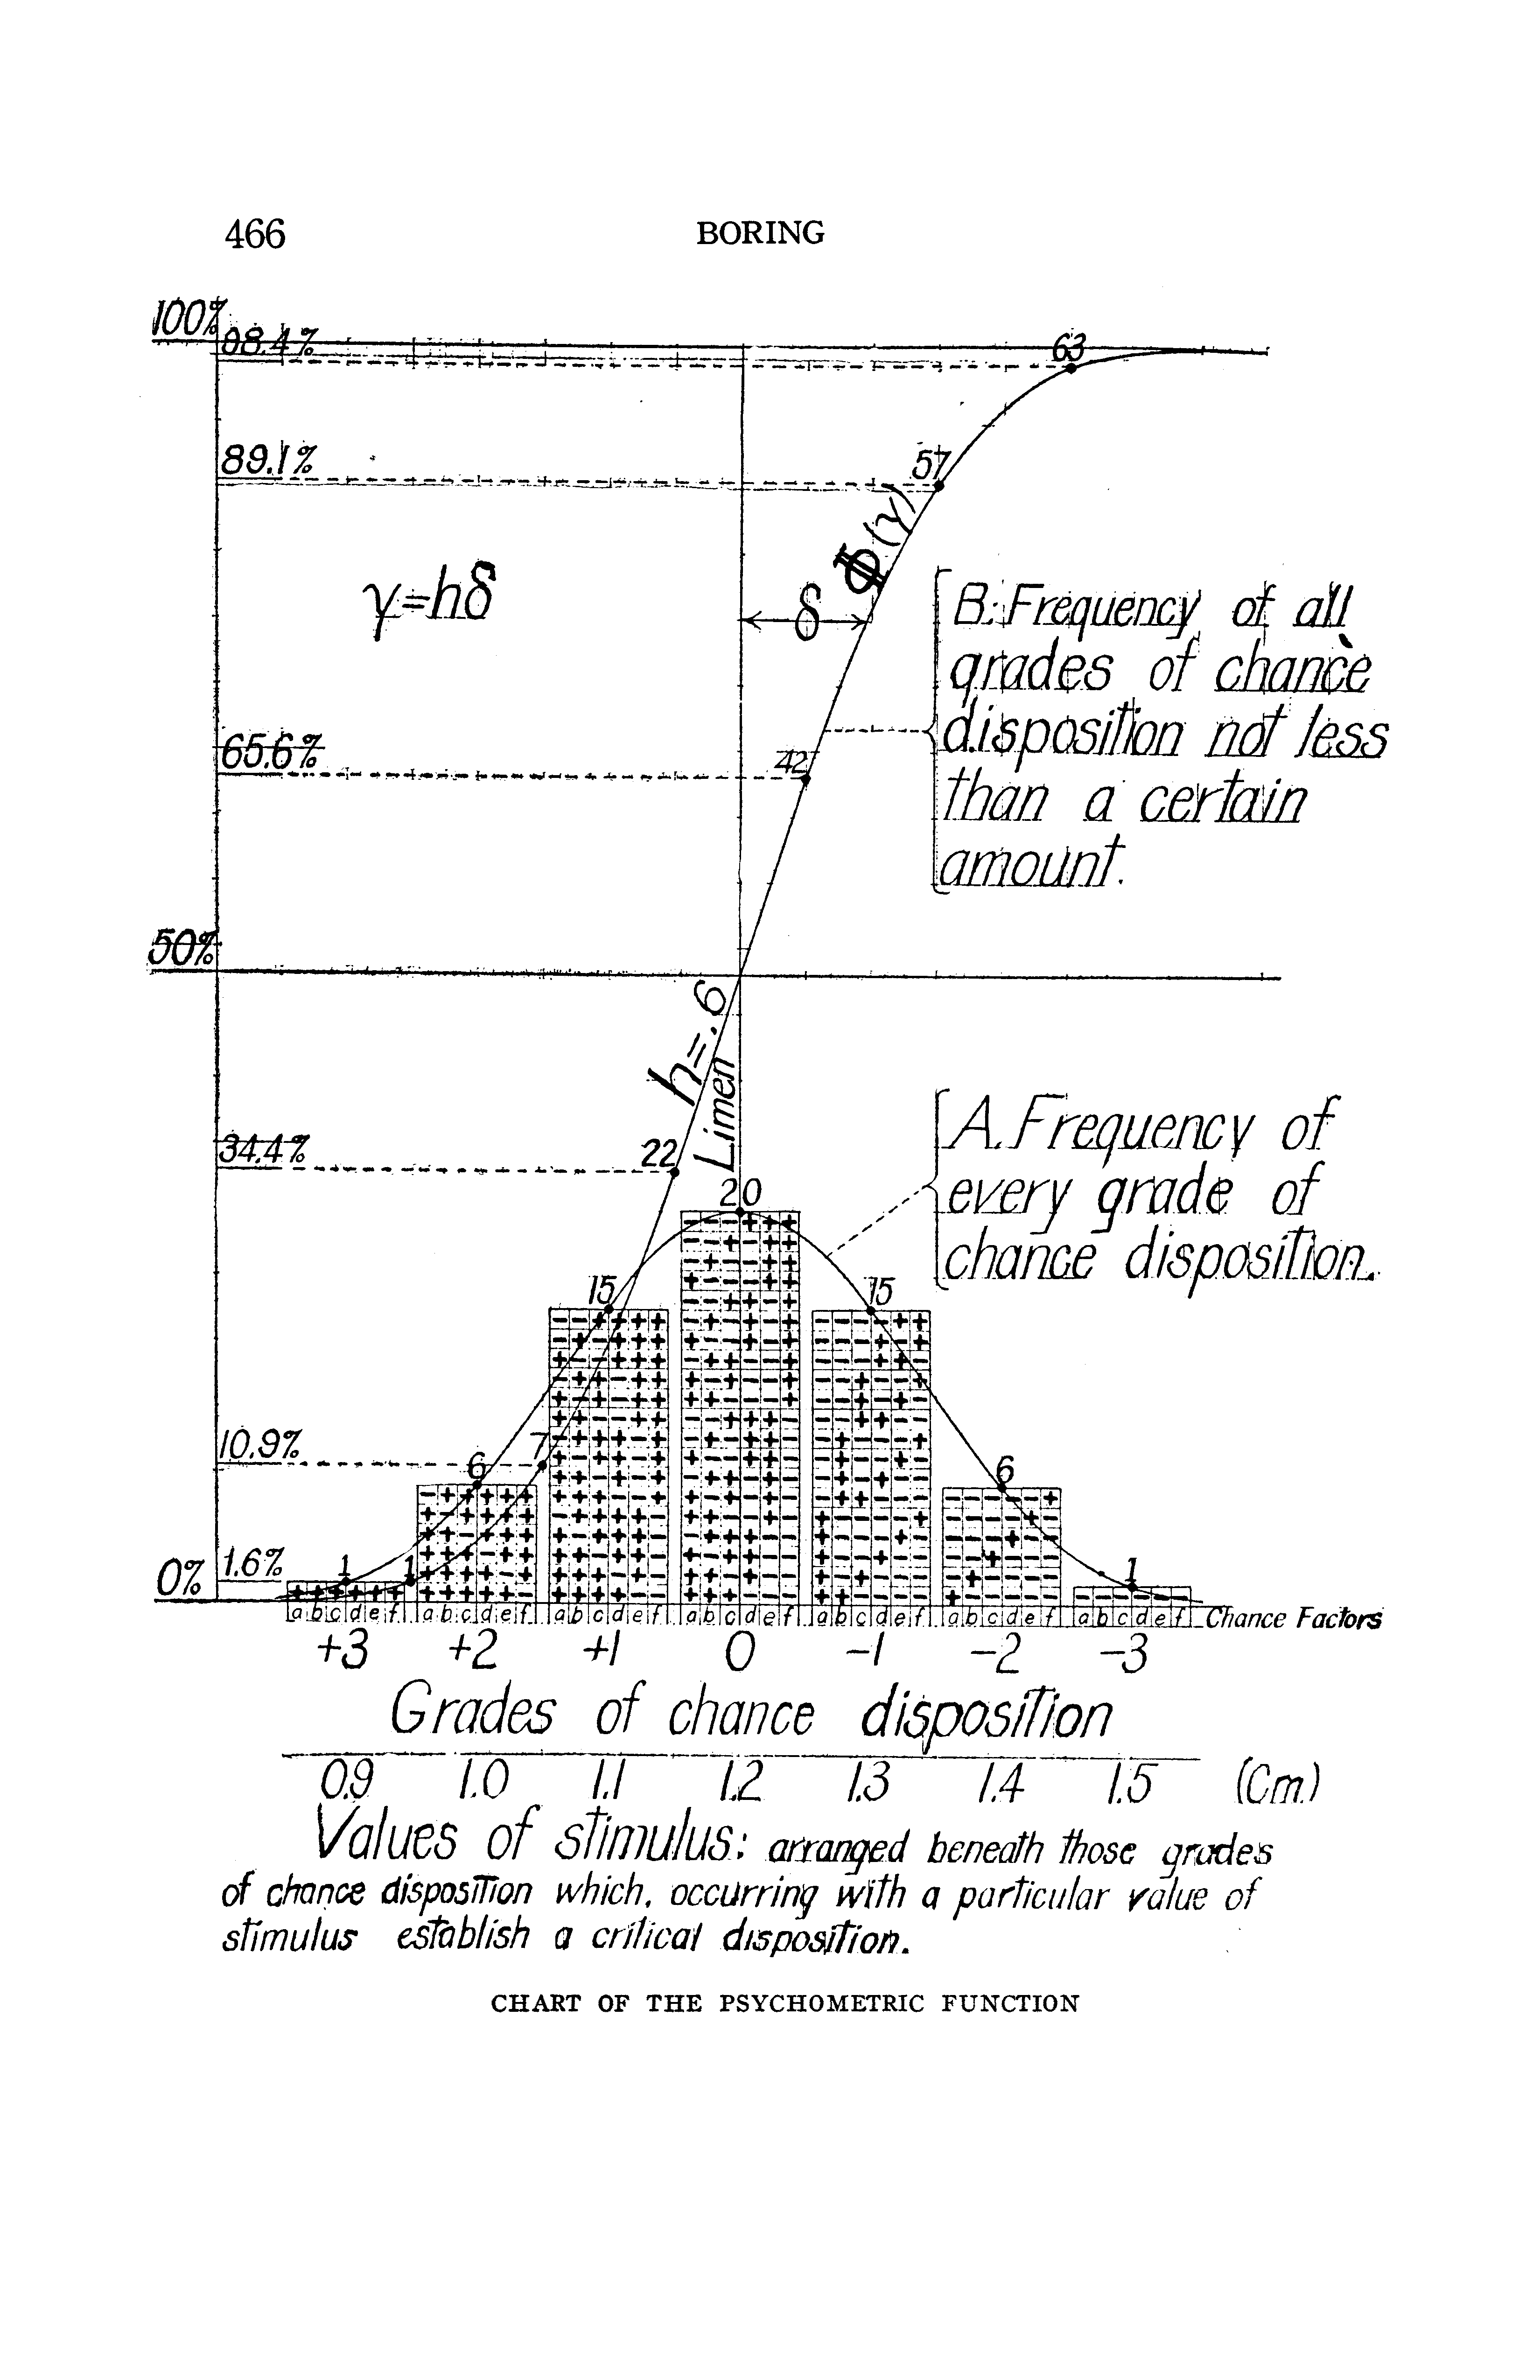
\includegraphics[width=0.85\linewidth]{figures/chart_of_pf} 

}

\caption{A chart of the psychometric function. The experiment in this paper places two points on a subject's skin separated by some distance, and has them answer their impression of whether there is one point or two, recorded as either 'two points' or 'not two points'. As the separation of aesthesiometer points increases, so too does the subject's confidence in their perception of 'two-ness'. So at what separation is the impression of two points liminal?}\label{fig:ch020-chart-of-pf}
\end{figure}

Figure \ref{fig:ch020-chart-of-pf} displays the key aspects of the psychometric function. The most crucial part is the sigmoid function, the S-like non-decreasing curve which in this case is represented by the Normal CDF, \(\Phi(\gamma)\). The horizontal axis represents the stimulus stimulus intensity, the separation of two points in centimeters. The vertical axis represents the probability that a subject has the impression of two points. With only experimental data, the response proportion becomes an approximation for the probability.

This leads me to talk about the type of psychometric experiment that this paper deals with called a \emph{temporal order judgment} (TOJ) experiment. The concept is that if there are two distinct stimuli occurring nearly simultaneously then our brains will bind them into a single percept (perceive them as happening simultaneously). Compensation for small temporal differences is beneficial for coherent multisensory experiences, particularly in visual-speech synthesis as it is necessary to maintain an accurate representation of the sources of multisensory events. The temporal asynchrony between stimuli is called the \emph{stimulus onset asynchrony} (SOA), and the range of SOAs for which sensory signals are integrated into a global percept is called the \emph{temporal binding window}. When the SOA grows too large then the brain segregates the two signals and the temporal order can be determined.

Our experiences in life as we age shape the mechanisms of processing multisensory signals, and some multisensory signals are integrated much more readily than others. Perceptual synchrony has been previously studied through the \emph{point of subjective simultaneity} (PSS) -- the temporal delay between two signals at which an observer is unsure about their temporal order \citep{stone2001now}. The temporal binding window is the time span over which sensory signals arising from different modalities appear integrated into a global percept. A deficit in temporal sensitivity may lead to a widening of the temporal binding window and reduce the ability to segregate unrelated sensory signals. In temporal order judgment tasks, the ability to discriminate the timing of multiple sensory signals is referred to as temporal sensitivity, and is studied through the measurement of the \emph{just noticeable difference} (JND) -- the smallest lapse in time so that a temporal order can just be determined. Figure \ref{fig:ch020-plot-ref-pf} highlights the features through which we study psychometric functions. The PSS is defined as the point where an observer can do no better at determining temporal order than random guessing (i.e.~the response probability is 50\%). The JND is defined as the extra temporal delay between stimuli so that the temporal order is just able to be determined. Historically this has been defined as the difference between the 84\% level\footnote{One standard deviation away from the mean in a Gaussian distribution.} and the PSS, though the upper level often depends on domain expertise.

\begin{figure}

{\centering 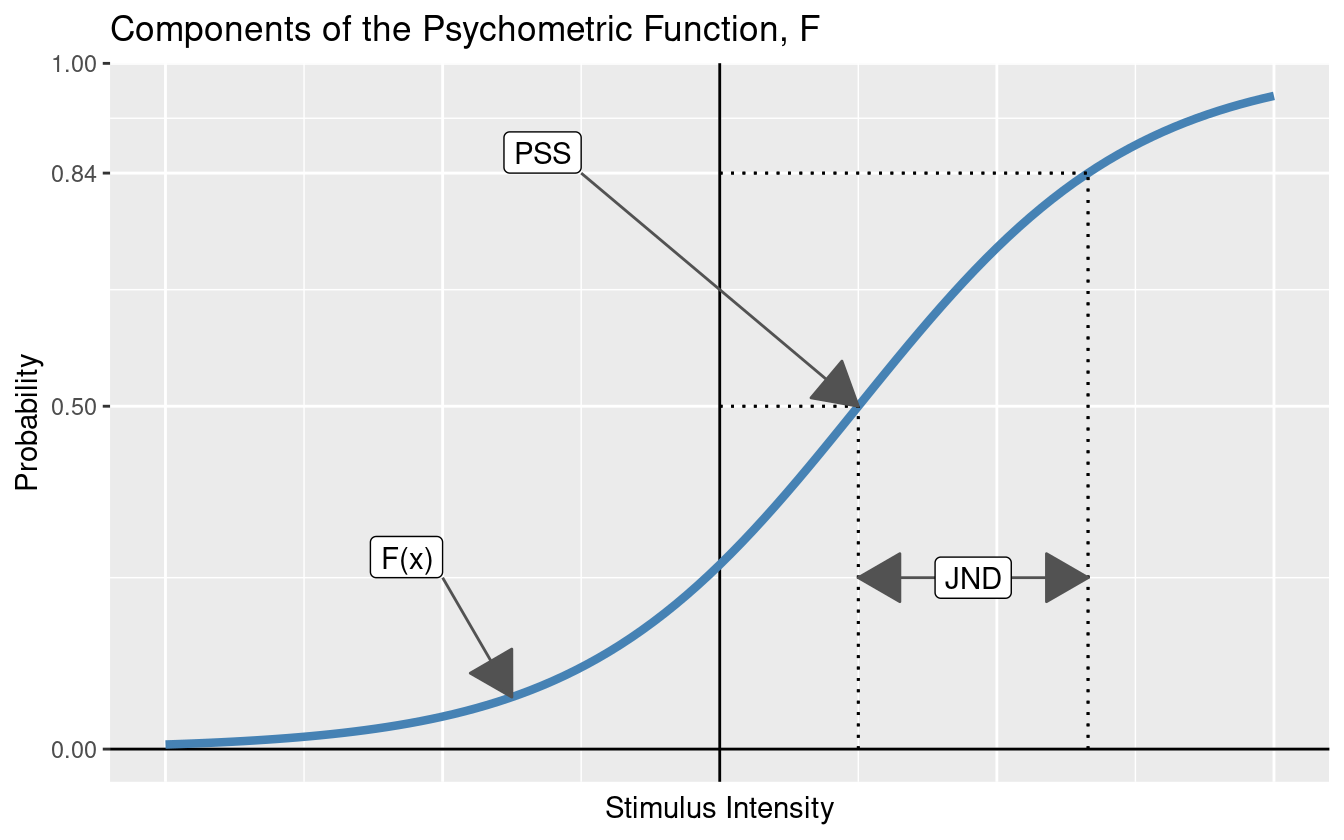
\includegraphics[width=0.85\linewidth]{020-psychometrics_files/figure-latex/ch020-plot-ref-pf-1} 

}

\caption{The PSS is defined as the point where an observer can do no better at determining temporal order than random guessing. The just noticeable difference is defined as the extra temporal delay between stimuli so that the temporal order is just able to be determined. Historically this has been defined as the difference between the 0.84 level and the PSS, though the upper level depends on domain expertise.}\label{fig:ch020-plot-ref-pf}
\end{figure}

Perceptual synchrony and temporal sensitivity can be modified through a baseline understanding. In order to perceive physical events as simultaneous, our brains must adjust for differences in temporal delays of transmission of both psychical signals and sensory processing \citep{fujisaki2004recalibration}. In some cases such as with audiovisual stimuli, the perception of simultaneity can be modified by repeatedly presenting the audiovisual stimuli at fixed time separations (called an adapter stimulus) to an observer \citep{vroomen2004recalibration}. This repetition of presenting the adapter stimulus is called \emph{temporal recalibration}.

The data set that I introduce in the next section concerns temporal order judgment across various sensory modalities with a temporal recalibration component.

\hypertarget{toj-task}{%
\section{Temporal Order Judgment Task}\label{toj-task}}

The data set that I am using in this paper comes from experiments done by A.N. Scurry and Dr.~F. Jiang in the Department of Psychology at the University of Nevada. Reduced temporal sensitivity in the aging population manifests in an impaired ability to perceive synchronous events as simultaneous, and similarly more difficulty in segregating asynchronous sensory signals that belong to different sources. The consequences of a widening of the temporal binding window is considered in \citet{scurry2019aging}, as well as a complete detailing of the experimental setup and recording process. A shortened summary of the methods is provided below.

There are four different tasks in the experiment: audio-visual, visual-visual, visual-motor, and duration, and I will refer to each task respectively as audiovisual, visual, sensorimotor, and duration. The participants consist of 15 young adults (age 20-27), 15 middle age adults (age 39-50), and 15 older adults (age 65-75), all recruited from the University of Nevada, Reno. Additionally all subjects are right handed and were reported to have normal or corrected to normal hearing and vision.

\begin{table}[!h]

\caption{\label{tab:ch020-multitask-data}Sample of motivating data.}
\centering
\begin{tabular}[t]{rrllllrl}
\toprule
soa & response & sid & task & trial & age\_group & age & sex\\
\midrule
-350 & 0 & O-m-BC & audiovisual & pre & older\_adult & 70 & M\\
-200 & 0 & M-m-SJ & duration & post1 & middle\_age & 48 & M\\
28 & 1 & O-f-KK & sensorimotor & pre & older\_adult & 66 & F\\
275 & 1 & O-f-MW & visual & post1 & older\_adult & 69 & F\\
\bottomrule
\end{tabular}
\end{table}

In the audiovisual TOJ task, participants were asked to determine the temporal order between an auditory and visual stimulus. Stimulus onset asynchrony values were selected uniformly between -500 to +500 ms with 50 ms steps, where negative SOAs indicated that the visual stimulus was leading, and positive values indicated that the auditory stimulus was leading. Each SOA value was presented 5 times in random order in the initial block. At the end of each trial the subject was asked to report if the auditory stimulus came before the visual, where a \(1\) indicates that they perceived the sound first, and a \(0\) indicates that they perceived the visual stimulus first.

A similar setup is repeated for the visual, sensorimotor, and duration tasks. The visual task presented two visual stimuli on the left and right side of a display with temporal asynchronies that varied between -300 ms to +300 ms with 25 ms steps. Negative SOAs indicated that the left stimulus was first, and positive that the right came first. A positive response indicates that the subject perceived the right stimulus first.

The sensorimotor task has subjects focus on a black cross on a screen. When it disappears, they respond by pressing a button. Additionally, when the cross disappears, a visual stimulus was flashed on the screen, and subjects were asked if they perceived the visual stimulus before or after their button press. The latency of the visual stimulus was partially determined by individual subject's average response time, so SOA values are not fixed between subjects and trials. A positive response indicates that the visual stimulus was perceived after the button press.

The duration task presents two vertically stacked circles on a screen with one appearing right after the other. The top stimulus appeared for a fixed amount of time of 300 ms, and the bottom was displayed for anywhere between +100 ms to +500 ms in 50 ms steps corresponding to SOA values between -200 ms to +200 ms. The subject then responds to if they perceived the bottom circle as appearing longer than the top circle.

\begin{table}[!h]

\caption{\label{tab:ch020-toj-summary}Summary of TOJ Tasks}
\centering
\begin{tabular}[t]{lll}
\toprule
Task & Positive Response & Positive SOA Truth\\
\midrule
Audiovisual & Perceived audio first & Audio came before visual\\
Visual & Perceived right first & Right came before left\\
Sensorimotor & Perceived visual first & Visual came before tactile\\
Duration & Perceived bottom as longer & Bottom lasted longer than top\\
\bottomrule
\end{tabular}
\end{table}

Finally, after the first block of each task was completed, the participants went through an adaptation period where they were presented with the respective stimuli from each task repeatedly at fixed temporal delays, then they repeated the task. To ensure that the adaptation affect persisted, the subject were presented with the adapter stimulus at regular intervals throughout the second block. The blocks are designated as \texttt{pre} and \texttt{post1}, \texttt{post2}, etc. in the data set. In this paper I will only be focusing on the \texttt{pre} and \texttt{post1} blocks.

\hypertarget{data-visualizations-and-quirks}{%
\section{Data Visualizations and Quirks}\label{data-visualizations-and-quirks}}

The dependent variable in these experiments is the perceived response which is encoded as a 0 or a 1, and the independent variable is the SOA value. If the response is plotted against the SOA values, then it is difficult to determine any relationship (see figure \ref{fig:ch020-simple-response-soa-plot}). Transparency can be used to better visualize the relationships between SOA value and responses. The center plot in figure \ref{fig:ch020-simple-response-soa-plot} uses the same data as the left plot, except that the transparency is set to 0.05. As a result, one can see that there is a higher density of ``0'' responses towards more negative SOAs, and a higher density of ``1'' responses for more positive SOAs. Taking it a step further, I can compute and plot the proportion of responses for a given SOA. This is displayed in the right panel. Now the relationship between SOA values and responses is clear -- as the SOA value goes from more negative to more positive, the proportion of positive responses increases from near 0 to near 1.

\begin{figure}

{\centering 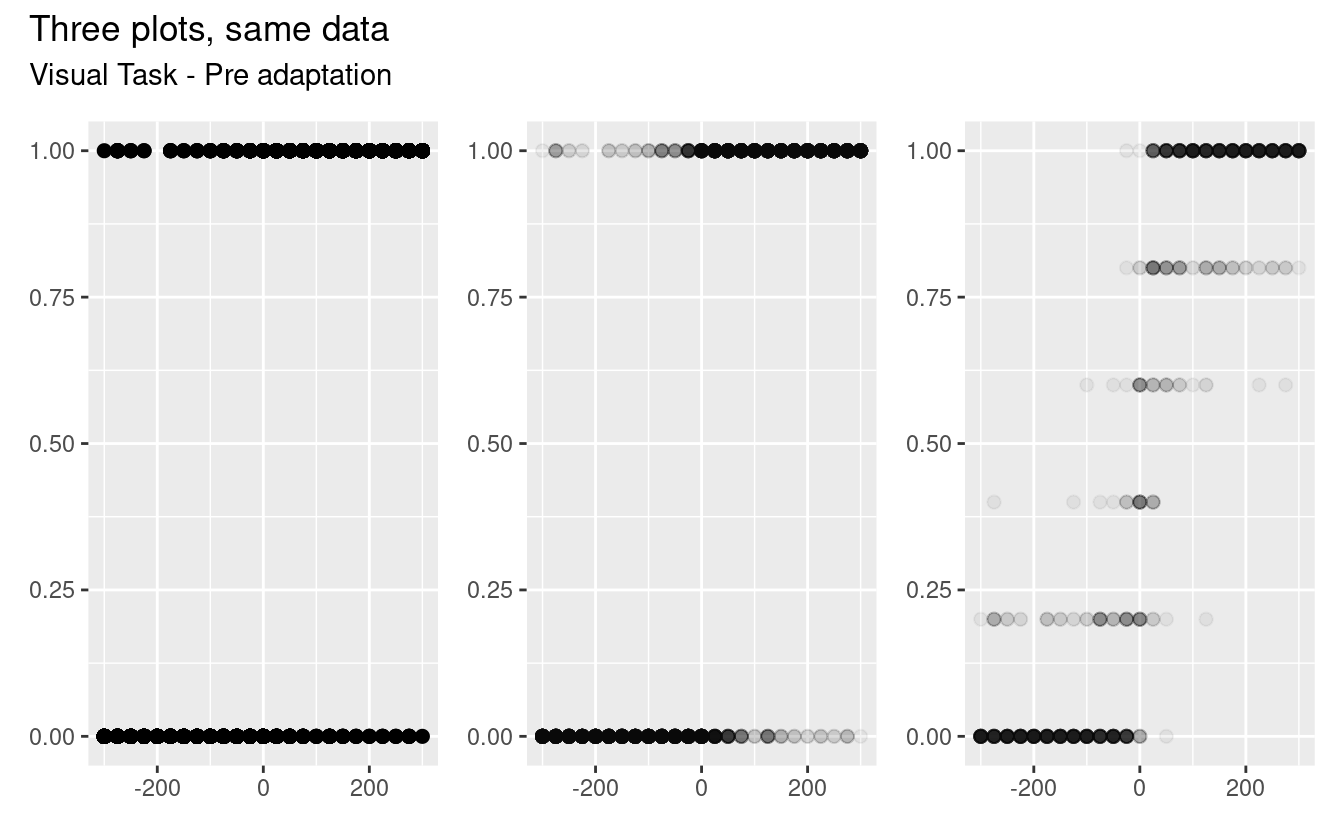
\includegraphics[width=0.85\linewidth]{020-psychometrics_files/figure-latex/ch020-simple-response-soa-plot-1} 

}

\caption{Left: Simple plot of response vs. soa value. Center: A plot of response vs. soa with transparency. Right: A plot of proportions vs. soa with transparency.}\label{fig:ch020-simple-response-soa-plot}
\end{figure}

Subjectively the right plot in figure \ref{fig:ch020-simple-response-soa-plot} is the easiest to interpret. Because of this, I will often present the observed and predicted data using the proportion of responses rather than the actual response. Proportional data also has the advantage of being bounded on the same interval as the response. For the audiovisual task, the responses can be aggregated into binomial data -- the number of positive responses for given SOA value -- which is sometimes more efficient to work with than the Bernoulli data (see table \ref{tab:ch020-av-bin-sample}). However the number of times an SOA is presented varies between the pre-adaptation and post-adaptation blocks; 5 and 3 times per SOA respectively.

\begin{table}[!h]

\caption{\label{tab:ch020-av-bin-sample}Audiovisual task with aggregated responses.}
\centering
\begin{tabular}[t]{lrrrr}
\toprule
trial & soa & n & k & proportion\\
\midrule
 & 200 & 5 & 4 & 0.80\\
\cmidrule{2-5}
 & 150 & 5 & 5 & 1.00\\
\cmidrule{2-5}
\multirow[t]{-3}{*}{\raggedright\arraybackslash pre} & -350 & 5 & 0 & 0.00\\
\cmidrule{1-5}
 & 350 & 3 & 3 & 1.00\\
\cmidrule{2-5}
 & -500 & 3 & 1 & 0.33\\
\cmidrule{2-5}
\multirow[t]{-3}{*}{\raggedright\arraybackslash post1} & -200 & 3 & 0 & 0.00\\
\bottomrule
\end{tabular}
\end{table}

Other quirks about the data pertain to the subjects. There is one younger subject that did not complete the audiovisual task, and one younger subject that did not complete the duration task. Additionally there is one older subject who's response data for the post-adaptation audiovisual task is unreasonable\footnote{By unreasonable, I mean that it is extremely unlikely that the data represents genuine responses.} (see figure \ref{fig:ch020-av-post1-O-f-CE-plot}).

\begin{figure}

{\centering 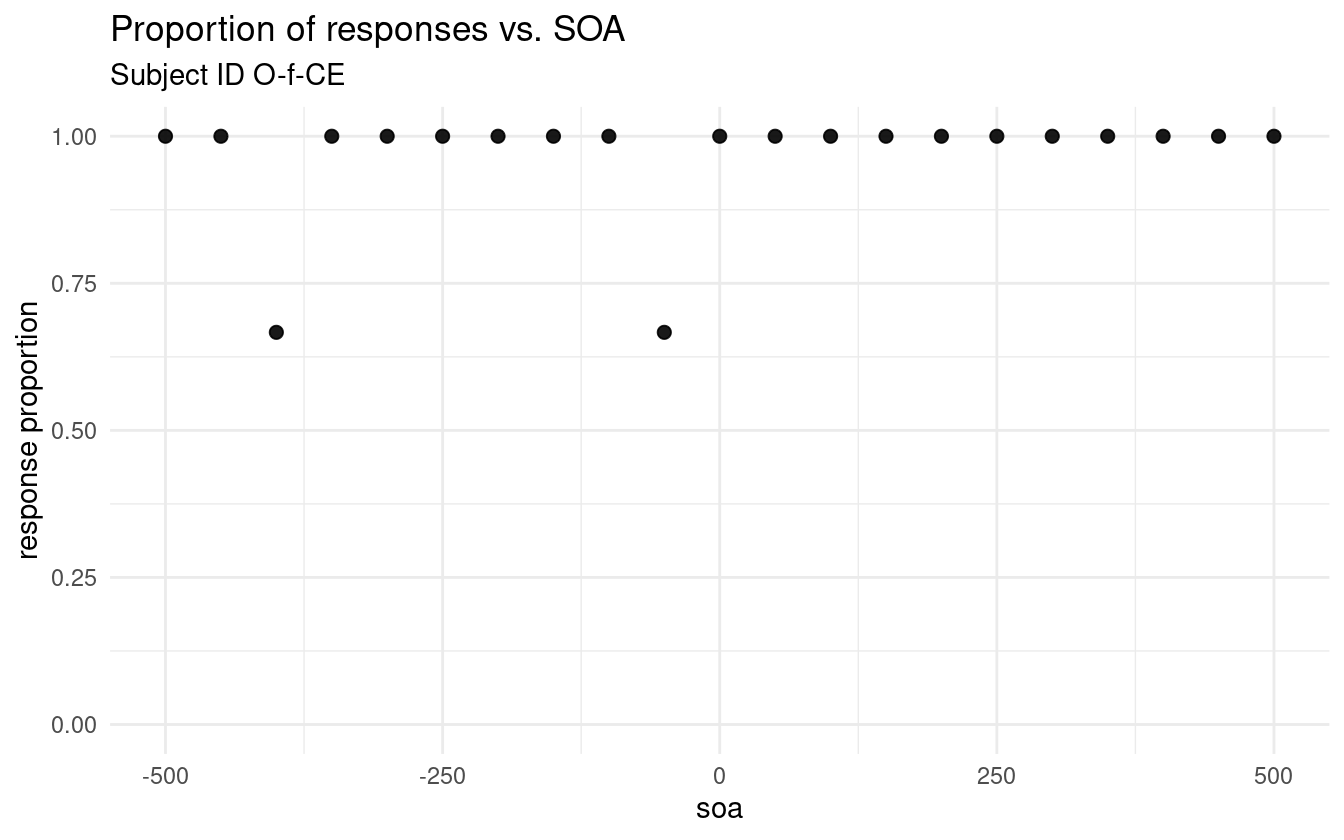
\includegraphics[width=0.85\linewidth]{020-psychometrics_files/figure-latex/ch020-av-post1-O-f-CE-plot-1} 

}

\caption{Post-adaptation response data for O-f-CE}\label{fig:ch020-av-post1-O-f-CE-plot}
\end{figure}

It is unreasonable because, of all the negative SOAs, there were only two correct responses\footnote{Correct in the sense that the perceived order matches the actual order.}. If a subject is randomly guessing the temporal order, then a naive estimate for the proportion of correct responses is 0.5. If a subject's proportion of correct responses is above 0.5, then they are doing better than random guessing. In figure \ref{fig:ch020-av-post-neg-trials} it is seen that subject O-f-CE is the only one who's proportion is below 0.5 (and by a considerable amount).

\begin{figure}

{\centering 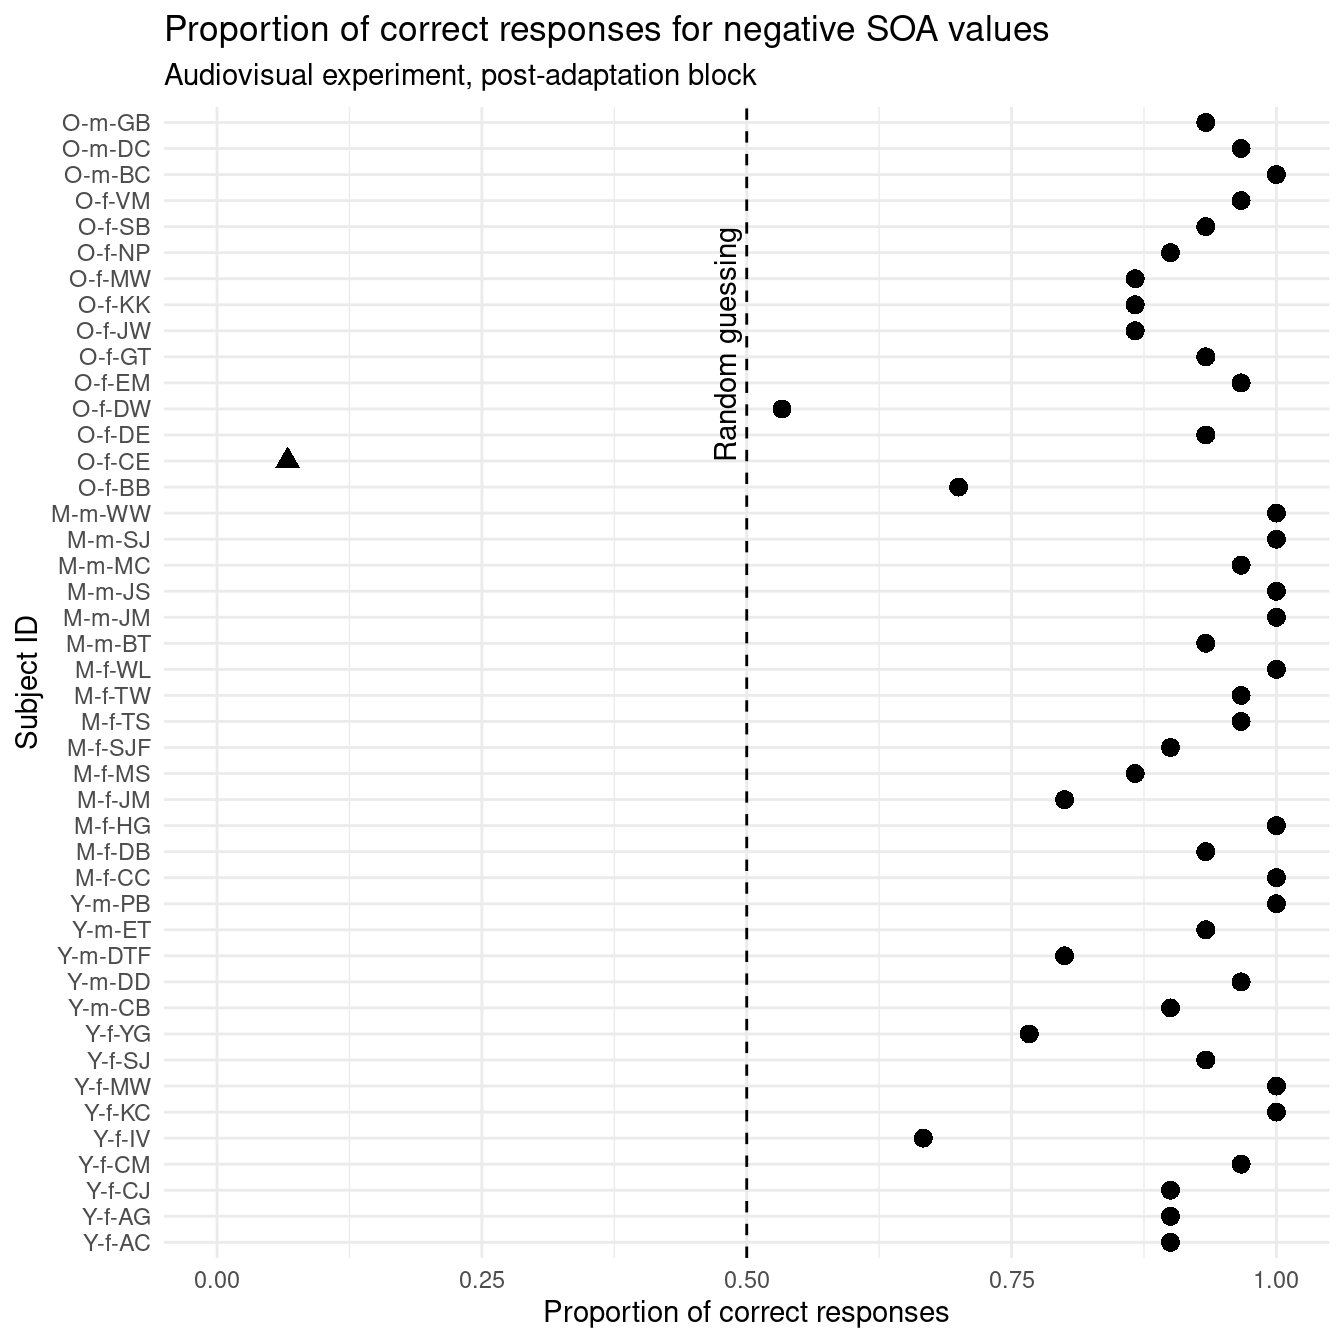
\includegraphics[width=0.85\linewidth]{020-psychometrics_files/figure-latex/ch020-av-post-neg-trials-1} 

}

\caption{Proportion of correct responses for negative SOA values during the post-adaptation audiovisual experiment.}\label{fig:ch020-av-post-neg-trials}
\end{figure}

The consequences of leaving in this experimental block in the data is considered in the \protect\hyperlink{results}{Chapter 6}, but it is a clear outlier that must be noted. When this method of detecting outliers is repeated for all tasks and blocks, then I end up with 17 records in total (see figure \ref{fig:ch020-naive-prop-outliers}), one of which is the aforementioned subject.

\begin{figure}

{\centering 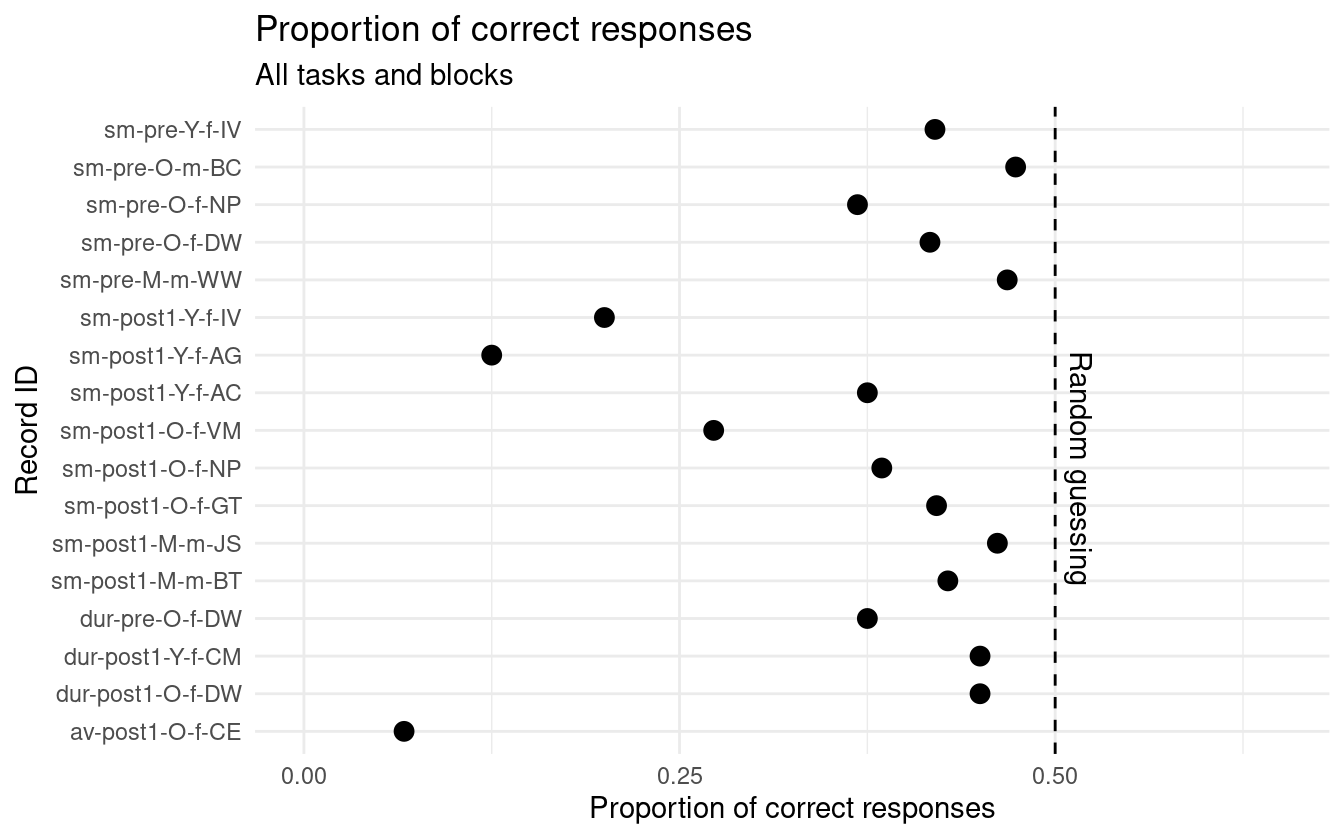
\includegraphics[width=0.85\linewidth]{020-psychometrics_files/figure-latex/ch020-naive-prop-outliers-1} 

}

\caption{Proportion of correct responses across all tasks and blocks Proportions are calculated individually for positive and negative SOAs.}\label{fig:ch020-naive-prop-outliers}
\end{figure}

Most of the records that are flagged by this method of outlier detection are from the sensorimotor task, and none are from the visual task. This may be attributed to the perceived difficulty of the task. One consequence of higher temporal sensitivity is that it is easier to determine temporal order. It may also be that determining temporal order is inherently easier for certain multisensory tasks compared to others. Since the sensorimotor task does not have fixed SOA values like the other tasks, it may be perceived as more difficult. Or perhaps the mechanisms that process tactile and visual signals are not as well coupled as those that process audio and visual signals. Once again, I'll consider the handling of the sensorimotor outliers in the results chapter.

Now that I have introduced the motivating data and some of the theory behind psychometric experiments, I am ready to introduce a Bayesian workflow for multilevel modeling of the psychometric function. If the reader is interested in a fun story, in the \protect\hyperlink{discussion}{discussion chapter} I talk about the process I went through to read in this psychometric data, clean it up, and produce a tidy data set that is ready for modeling. While data cleaning and transforming is a topic entirely to itself, it is not the main focus of this paper.

\hypertarget{methods}{%
\chapter{Methods}\label{methods}}

\hypertarget{model-development}{%
\section{Model Development}\label{model-development}}

\hypertarget{model-fitting}{%
\section{Model Fitting}\label{model-fitting}}

\hypertarget{model-checking}{%
\section{Model Checking}\label{model-checking}}

\hypertarget{predictive-performance}{%
\section{Predictive Performance}\label{predictive-performance}}

\hypertarget{model-development-1}{%
\chapter{Model Development}\label{model-development-1}}

\hypertarget{iter1}{%
\section{Iteration 1}\label{iter1}}

\textbf{Pre-Model, Pre-Data}

\emph{Conceptual Analysis}

\emph{Define Observational Space}

\emph{Construct Summary Statistics}

\textbf{Post-Model, Pre-Data}

\emph{Develop Model}

\emph{Construct Summary Functions}

\emph{Simulate Bayesian Ensemble}

\emph{Prior Checks}

\emph{Configure Algorithm}

\emph{Fit Simulated Ensemble}

\emph{Algorithmic Calibration}

\emph{Inferential Calibration}

\textbf{Post-Model, Post-Data}

\emph{Fit Observed Data}

\emph{Diagnose Posterior Fit}

\emph{Posterior Retrodictive Checks}

\emph{Celebrate}

\hypertarget{iter2}{%
\section{Iteration 2}\label{iter2}}

\textbf{Pre-Model, Pre-Data}

\emph{Conceptual Analysis}

\emph{Define Observational Space}

\emph{Construct Summary Statistics}

\textbf{Post-Model, Pre-Data}

\emph{Develop Model}

\emph{Construct Summary Functions}

\emph{Simulate Bayesian Ensemble}

\emph{Prior Checks}

\emph{Configure Algorithm}

\emph{Fit Simulated Ensemble}

\emph{Algorithmic Calibration}

\emph{Inferential Calibration}

\textbf{Post-Model, Post-Data}

\emph{Fit Observed Data}

\emph{Diagnose Posterior Fit}

\emph{Posterior Retrodictive Checks}

\emph{Celebrate}

\hypertarget{iter3}{%
\section{Iteration 3}\label{iter3}}

\textbf{Pre-Model, Pre-Data}

\emph{Conceptual Analysis}

\emph{Define Observational Space}

\emph{Construct Summary Statistics}

\textbf{Post-Model, Pre-Data}

\emph{Develop Model}

\emph{Construct Summary Functions}

\emph{Simulate Bayesian Ensemble}

\emph{Prior Checks}

\emph{Configure Algorithm}

\emph{Fit Simulated Ensemble}

\emph{Algorithmic Calibration}

\emph{Inferential Calibration}

\textbf{Post-Model, Post-Data}

\emph{Fit Observed Data}

\emph{Diagnose Posterior Fit}

\emph{Posterior Retrodictive Checks}

\emph{Celebrate}

\hypertarget{iter4}{%
\section{Iteration 4}\label{iter4}}

\textbf{Pre-Model, Pre-Data}

\emph{Conceptual Analysis}

\emph{Define Observational Space}

\emph{Construct Summary Statistics}

\textbf{Post-Model, Pre-Data}

\emph{Develop Model}

\emph{Construct Summary Functions}

\emph{Simulate Bayesian Ensemble}

\emph{Prior Checks}

\emph{Configure Algorithm}

\emph{Fit Simulated Ensemble}

\emph{Algorithmic Calibration}

\emph{Inferential Calibration}

\textbf{Post-Model, Post-Data}

\emph{Fit Observed Data}

\emph{Diagnose Posterior Fit}

\emph{Posterior Retrodictive Checks}

\emph{Celebrate}

\hypertarget{iter5}{%
\section{Iteration 5}\label{iter5}}

\textbf{Pre-Model, Pre-Data}

\emph{Conceptual Analysis}

\emph{Define Observational Space}

\emph{Construct Summary Statistics}

\textbf{Post-Model, Pre-Data}

\emph{Develop Model}

\emph{Construct Summary Functions}

\emph{Simulate Bayesian Ensemble}

\emph{Prior Checks}

\emph{Configure Algorithm}

\emph{Fit Simulated Ensemble}

\emph{Algorithmic Calibration}

\emph{Inferential Calibration}

\textbf{Post-Model, Post-Data}

\emph{Fit Observed Data}

\emph{Diagnose Posterior Fit}

\emph{Posterior Retrodictive Checks}

\emph{Celebrate}

\hypertarget{results}{%
\chapter{Psychometric Results}\label{results}}

What was the point of going through all the work of building a model if not to answer the questions that motivated the model in the first place? To reiterate, the questions pertain to how the brain reconciles stimuli originating from different sources, and if biological (age) and contextual (task, temporal recalibration) factors contribute to global percepts. The way through which these questions are answered is through a psychometric experiment and the resulting psychometric function (\protect\hyperlink{motivating-data}{chapter 2}). I've divided this chapter into two sections - the affects of temporal recalibration and the consideration of a lapse rate. Temporal recalibration is considered in the context of perceptual synchrony and temporal sensitivity, and the results are broken down by age group. Also recall that there are four separate tasks - audiovisual, visual, duration, and sensorimotor.

Temporal recalibration consists of presenting a subject with an adapting stimulus throughout a block of a psychometric experiment. Depending on the mechanisms at work, the resulting psychometric function can either be shifted (biased) towards the adapting stimulus (lag adaption) or away (Bayesian adaptation). The theory of integrating sensory signals is beyond the scope of this paper, but some papers discussing sensory adaptation in more detail are \citet{miyazaki2006bayesian}, \citet{sato2011bayesian}, and \citet{stocker2005sensory}. The statistical associations are reported without consideration for the deeper psychological theory.

\hypertarget{on-perceptual-synchrony}{%
\section{On Perceptual Synchrony}\label{on-perceptual-synchrony}}

Perceptual synchrony is when the temporal delay between two stimuli is small enough so that the brain integrates the two signals into a global percept - perceived as happening simultaneously. Perceptual synchrony is studied through the point of subjective simultaneity (PSS), and in a simple sense represents the bias towards a given stimulus. Ideally the bias would be zero, but human perception is liable to change due to every day experiences. The pre-adaptation block is a proxy for implicit bias, and the post-adaptation indicates whether lag or Bayesian adaptation is taking place. Some researchers believe that both forms of adaptation are taking place at all times and that the mixture rates are determined by biological and contextual factors. I will try to stay away from making any strong determinations and will only present the results conditional on the model and the data.

\textbf{Audiovisual TOJ Task}

There are two ways that we can visually draw inferences across the 6 different age-block combinations. The distributions can either be faceted by age group, or they can be faceted by block. There are actually many ways that the data can be presented, but these two methods of juxtaposition help to answer two questions - how does the effect of adaptation vary by age group, and is there a difference in age groups by block? The left hand plot of figure \ref{fig:ch050-Eastern-Cat} answers the former, and the right hand plot answers the latter.

\begin{figure}

{\centering 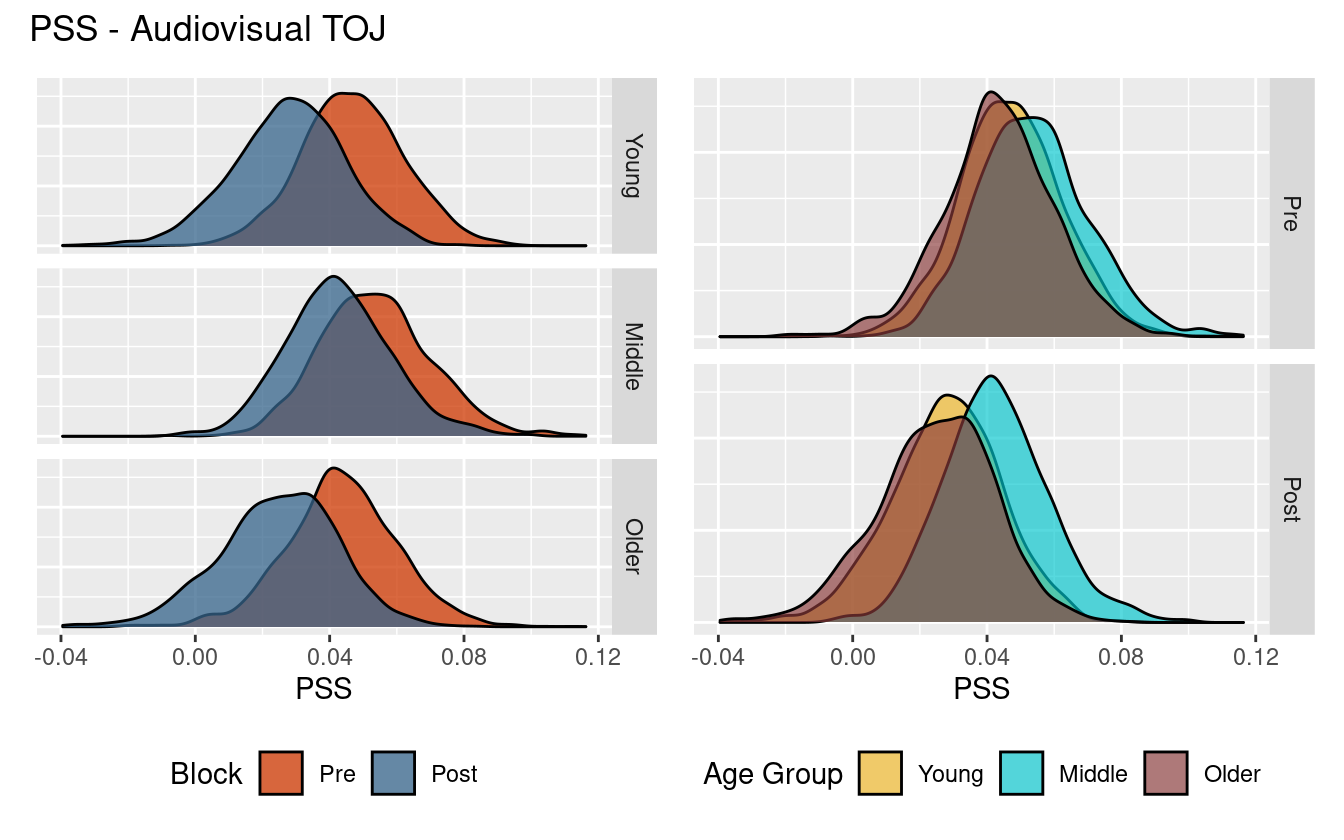
\includegraphics[width=0.85\linewidth]{050-results_files/figure-latex/ch050-Eastern-Cat-1} 

}

\caption{Posterior distribution of PSS values for the audiovisual task.}\label{fig:ch050-Eastern-Cat}
\end{figure}

Across all age groups, temporal recalibration results in a negative shift towards zero in the PSS (as shown by the left hand plot), but there is no significant difference in the PSS between age groups (right hand plot). A very convenient consequence of using MCMC is that the samples from the posterior can be recombined in many ways to describe new phenomena. The PSS values can even be pooled across age groups so that the marginal affect of recalibration may be considered (left hand plot of figure \ref{fig:ch050-Beta-Lonesome}).

\begin{figure}

{\centering 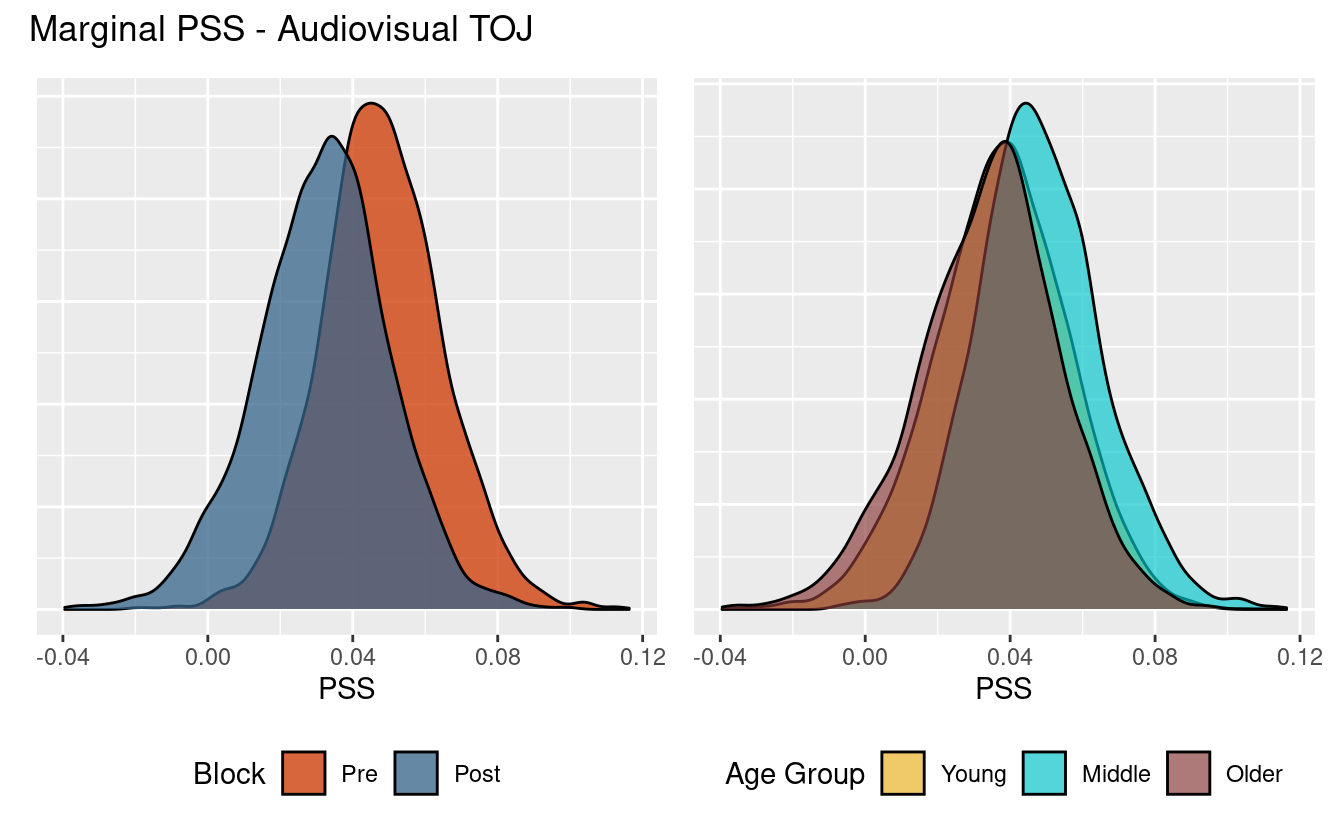
\includegraphics[width=0.85\linewidth]{050-results_files/figure-latex/ch050-Beta-Lonesome-1} 

}

\caption{Posterior distribution of PSS values for the audiovisual task. Left: Marginal over age group. Right: Marginal over block.}\label{fig:ch050-Beta-Lonesome}
\end{figure}

Now with the marginal of age group, the distribution of differences between pre- and post-adaptation blocks can be calculated. I could report a simple credible interval, but it almost seems disingenuous given that the entire distribution is available. I could report that the \(90\%\) highest posterior density interval (HPDI) of the difference is \((-0.036, 0.003)\), but consider the following figure instead.

\begin{figure}

{\centering 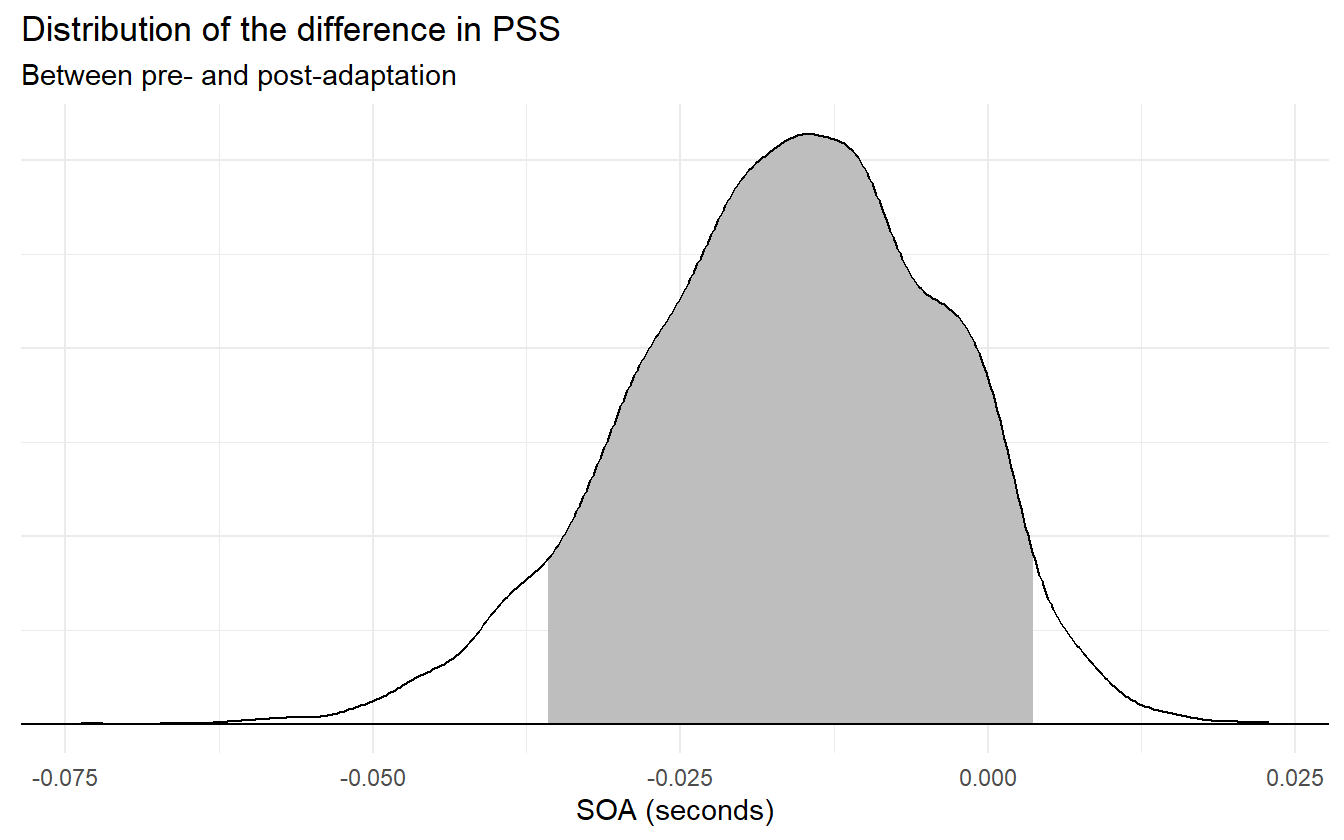
\includegraphics[width=0.85\linewidth]{050-results_files/figure-latex/ch050-Omega-Permanent-1} 

}

\caption{Distribution of differences for pre- and post-adaptation PSS values with 90\% HPDI.}\label{fig:ch050-Omega-Permanent}
\end{figure}

Figure \ref{fig:ch050-Omega-Permanent} shows the distribution of differences with the \(90\%\) HPDI region shaded. From this figure, one might conclude that the effect of recalibration, while small, is still noticeable for the audiovisual task. While this could be done for every task in the rest of this chapter, I do not think it is worth repeating as I am not trying to prove anything about the psychometric experiment itself (that is for a later paper). The point of this demonstration is simply that it can be done (and easily), and how to summarize the data both visually and quantitatively.

\textbf{Visual TOJ Task}

\begin{figure}

{\centering 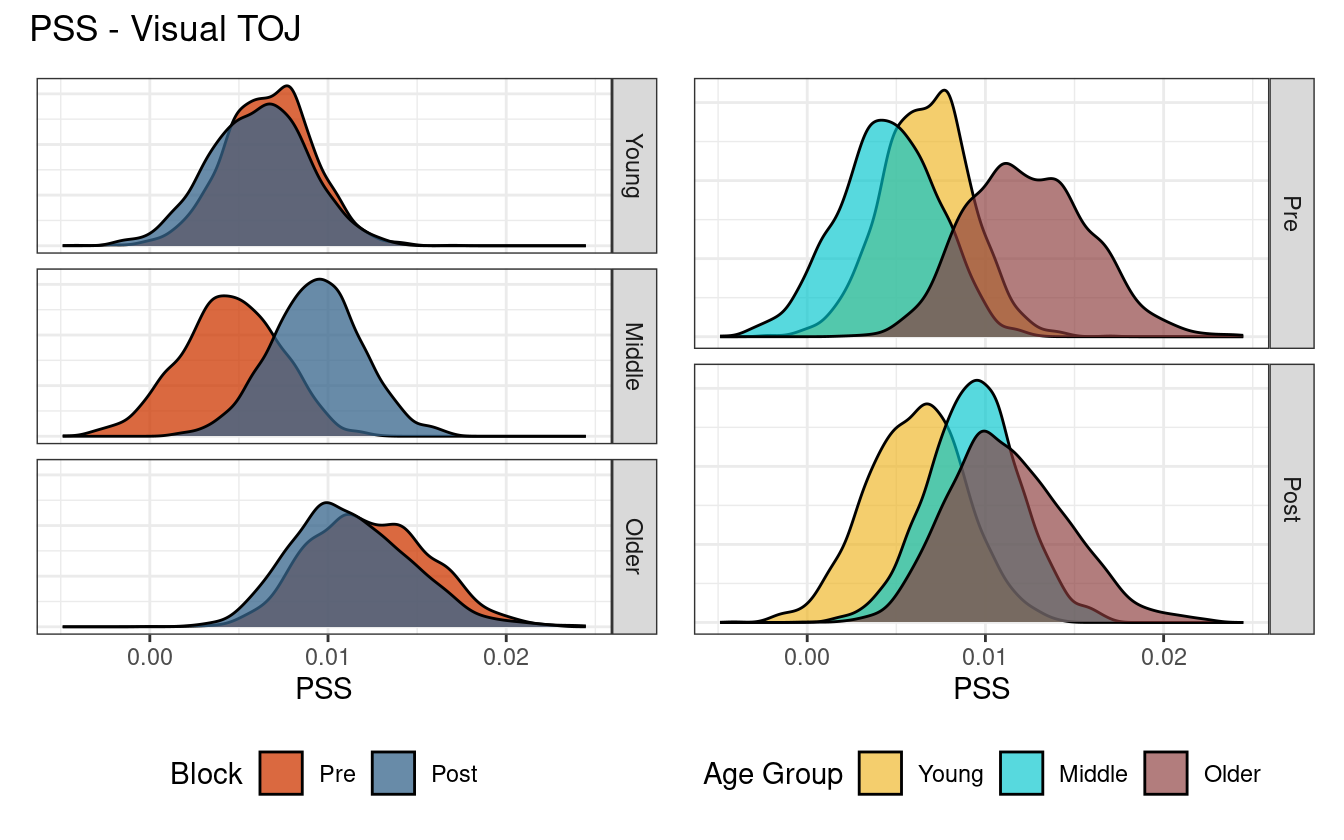
\includegraphics[width=0.85\linewidth]{050-results_files/figure-latex/ch050-Gruesome-Waffle-1} 

}

\caption{Posterior distribution of PSS values for the visual task.}\label{fig:ch050-Gruesome-Waffle}
\end{figure}

Here there is no clear determination if recalibration has an effect on perceptual synchrony, as it is only the middle age group that shows a shift in bias. Even more, there is a lot of overlap between age group. Looking at the marginal distributions (figure \ref{fig:ch050-Cold-Gamma}), there may be a difference between the younger and older age groups, and the middle age and older age groups.

\begin{figure}

{\centering 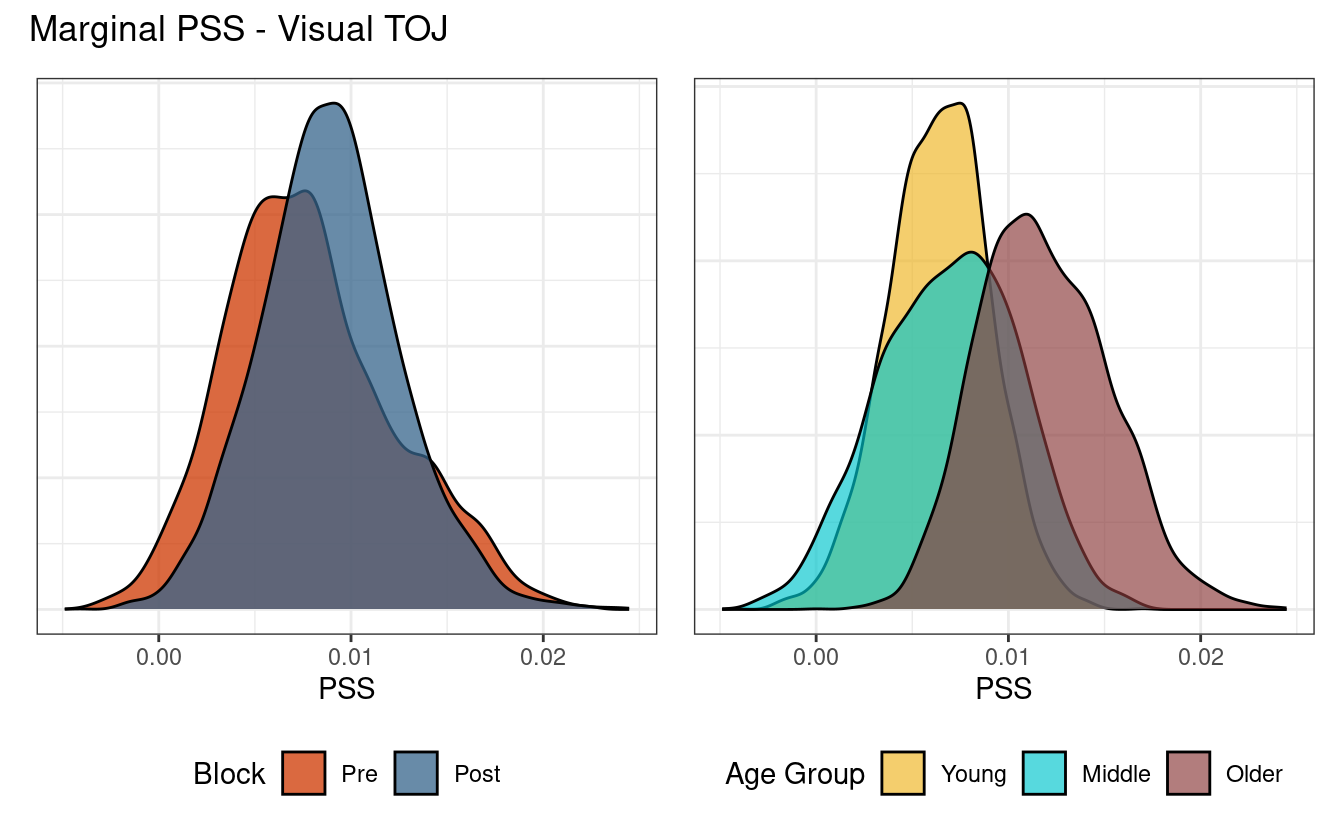
\includegraphics[width=0.85\linewidth]{050-results_files/figure-latex/ch050-Cold-Gamma-1} 

}

\caption{The difference between the older age group and the two others is noticeable, but not likely significant.}\label{fig:ch050-Cold-Gamma}
\end{figure}

These plots are useful for quickly being able to determine if there is a difference in factors. If there is a suspected difference, then the distribution can be calculated from the posterior samples as needed. I suspect that there may be a difference between the older age group and the other two, so I calculated the differences, and summarize them with the histogram in figure \ref{fig:ch050-Rapid-Postal}.

\begin{figure}

{\centering 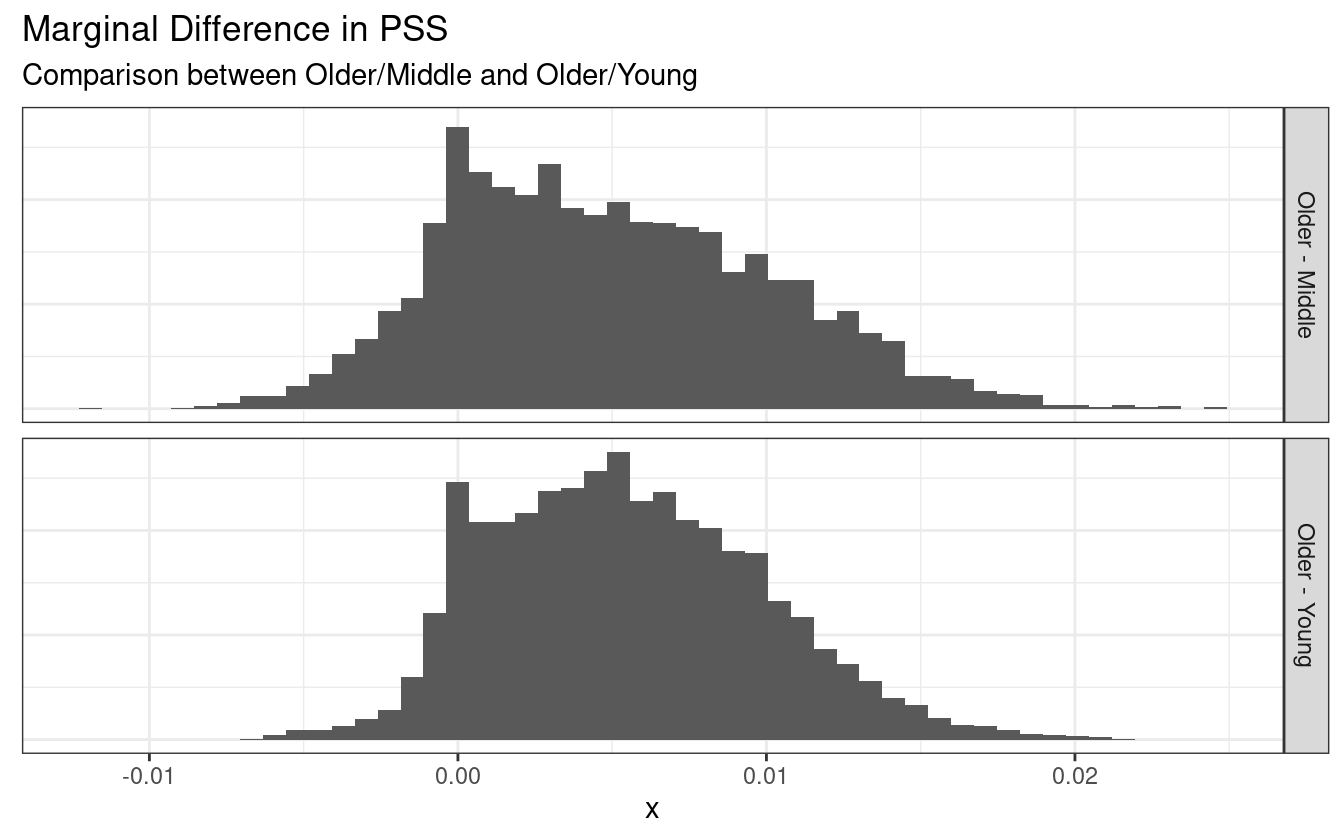
\includegraphics[width=0.85\linewidth]{050-results_files/figure-latex/ch050-Rapid-Postal-1} 

}

\caption{The bulk of the distribution is above zero, but there is still a chance that there is no difference in the distribution of PSS values between the age groups during the visual TOJ experiment.}\label{fig:ch050-Rapid-Postal}
\end{figure}

The bulk of the distribution is above zero, but there is still a chance that there is no difference in the distribution of PSS values between the age groups during the visual TOJ experiment.

\textbf{Duration TOJ Task}

\begin{figure}

{\centering 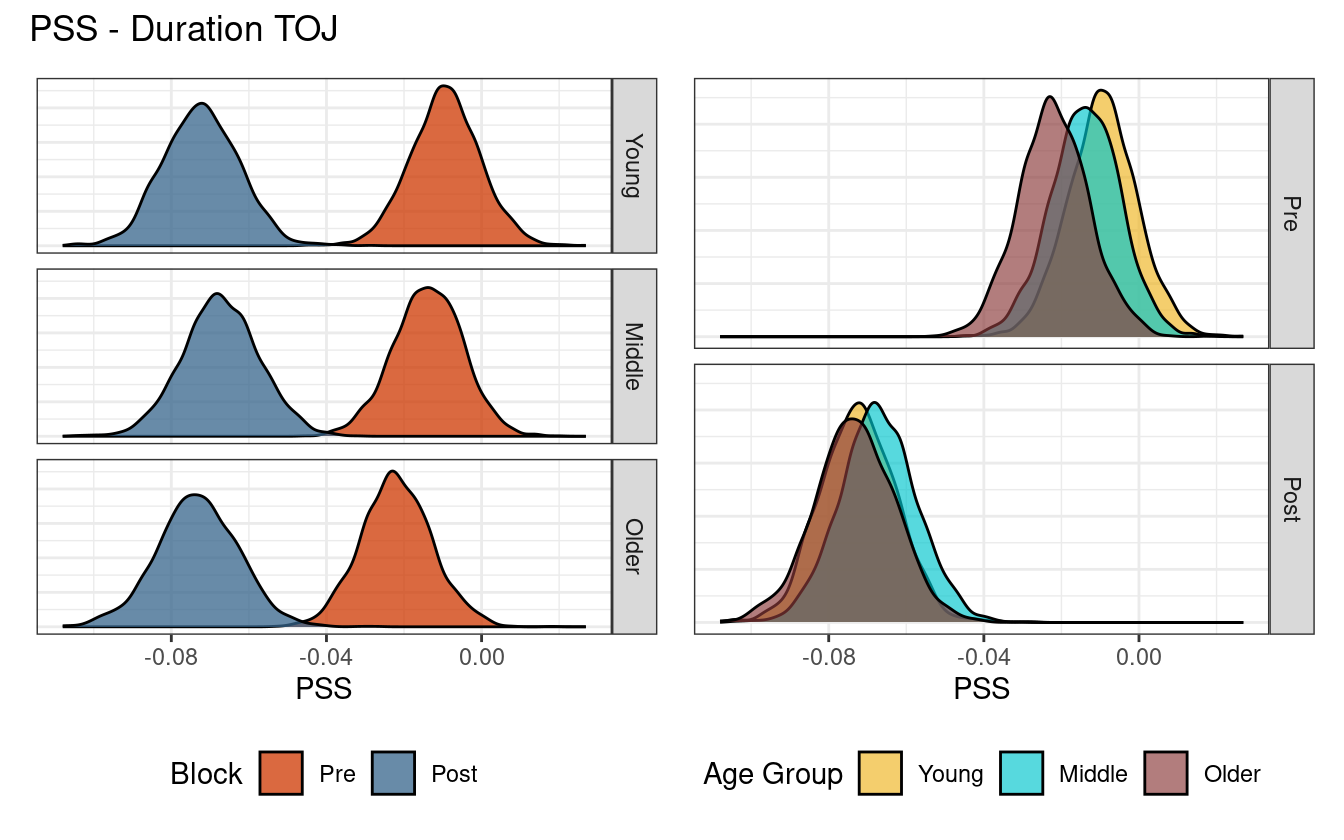
\includegraphics[width=0.85\linewidth]{050-results_files/figure-latex/ch050-Stormy-Frostbite-1} 

}

\caption{Posterior distribution of PSS values for the duration task.}\label{fig:ch050-Stormy-Frostbite}
\end{figure}

The duration TOJ task is very interesting because 1) recalibration had a visually significant effect across all age groups, and 2) there is virtually no difference between the age groups. I could plot the marginal distribution, but it wouldn't likely give any more insight. What I might ask is what is it about the duration task that lets temporal recalibration have such a significant effect? Is human perception of time duration more malleable than our perception to other sensory signals?

\textbf{Sensorimotor TOJ Task}

\begin{figure}

{\centering 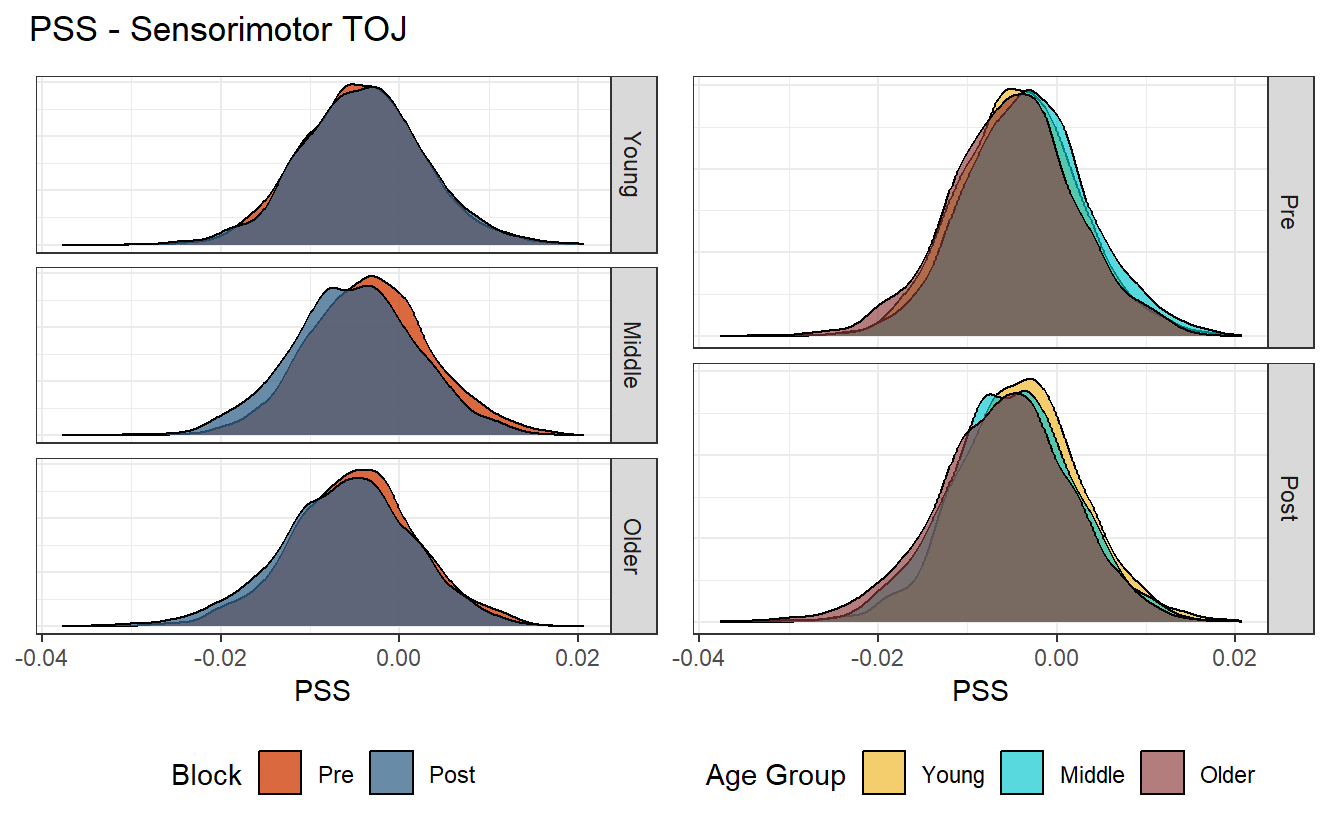
\includegraphics[width=0.85\linewidth]{050-results_files/figure-latex/ch050-Homeless-Anaconda-1} 

}

\caption{Posterior distribution of PSS values for the sensorimotor task.}\label{fig:ch050-Homeless-Anaconda}
\end{figure}

There are no differences between age groups or blocks when it comes to perceptual synchrony in the sensorimotor task.

\hypertarget{on-temporal-sensitivity}{%
\section{On Temporal Sensitivity}\label{on-temporal-sensitivity}}

Temporal sensitivity is the ability to successfully integrate signals arising from the same event, or segregate signals from different events. When the stimulus onset asynchrony increases, the ability to bind the signals into a single percept is reduced until they are perceived as distinct events with a temporal order. Those that are more readily able to determine temporal order have a higher temporal sensitivity, and it is measured through the slope of a psychometric function - specifically the quantity known as the just noticeable difference.

\textbf{Audiovisual TOJ Task}

\begin{figure}

{\centering 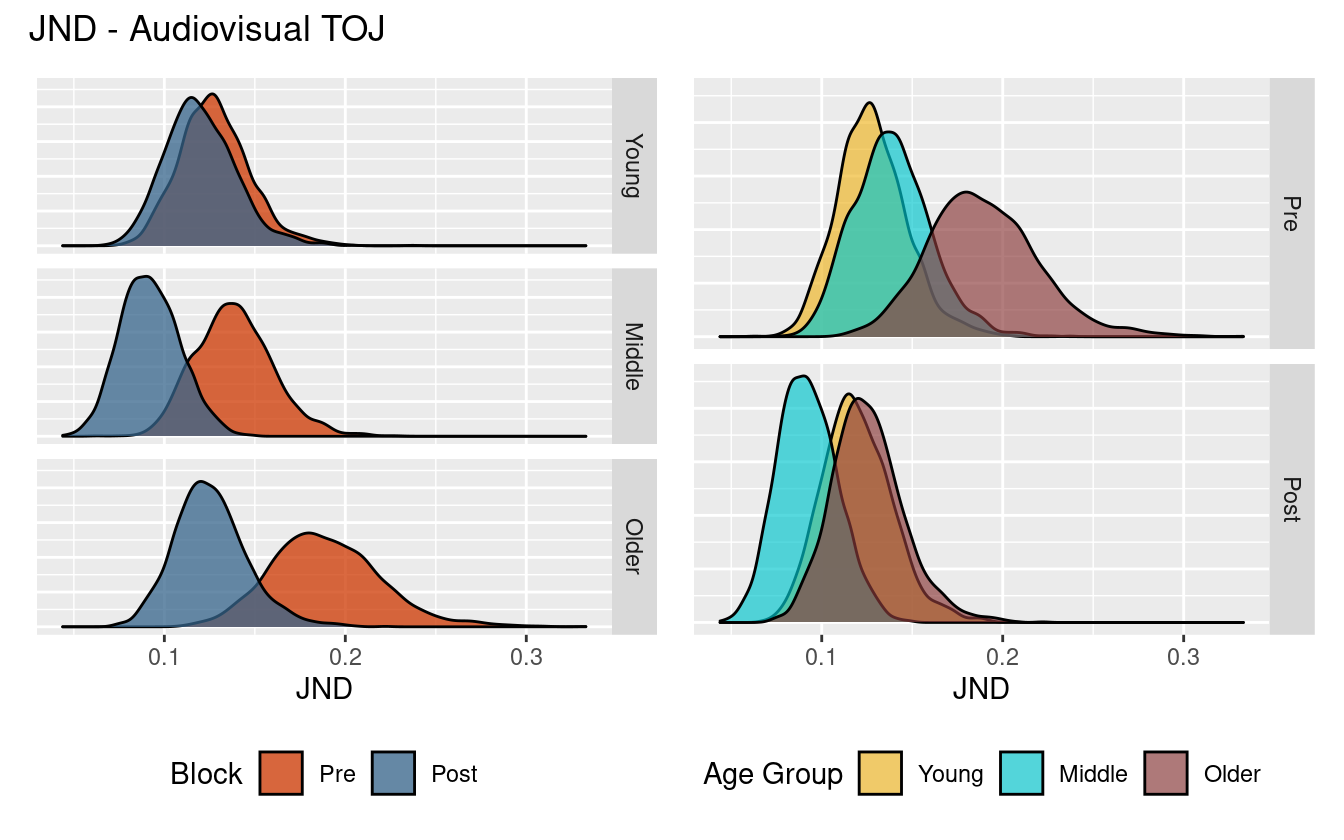
\includegraphics[width=0.85\linewidth]{050-results_files/figure-latex/ch050-Timely-Toupee-1} 

}

\caption{Posterior distribution of JND values for the audiovisual task.}\label{fig:ch050-Timely-Toupee}
\end{figure}

All age groups experienced an increase in temporal sensitivity, but the effect is largest in the older age group which also had the largest pre-adaptation JND estimates. There also appears to be some distinction between the older age group and the younger ones in the pre-adaptation block, but recalibration closes the gap.

\textbf{Visual TOJ Task}

\begin{figure}

{\centering 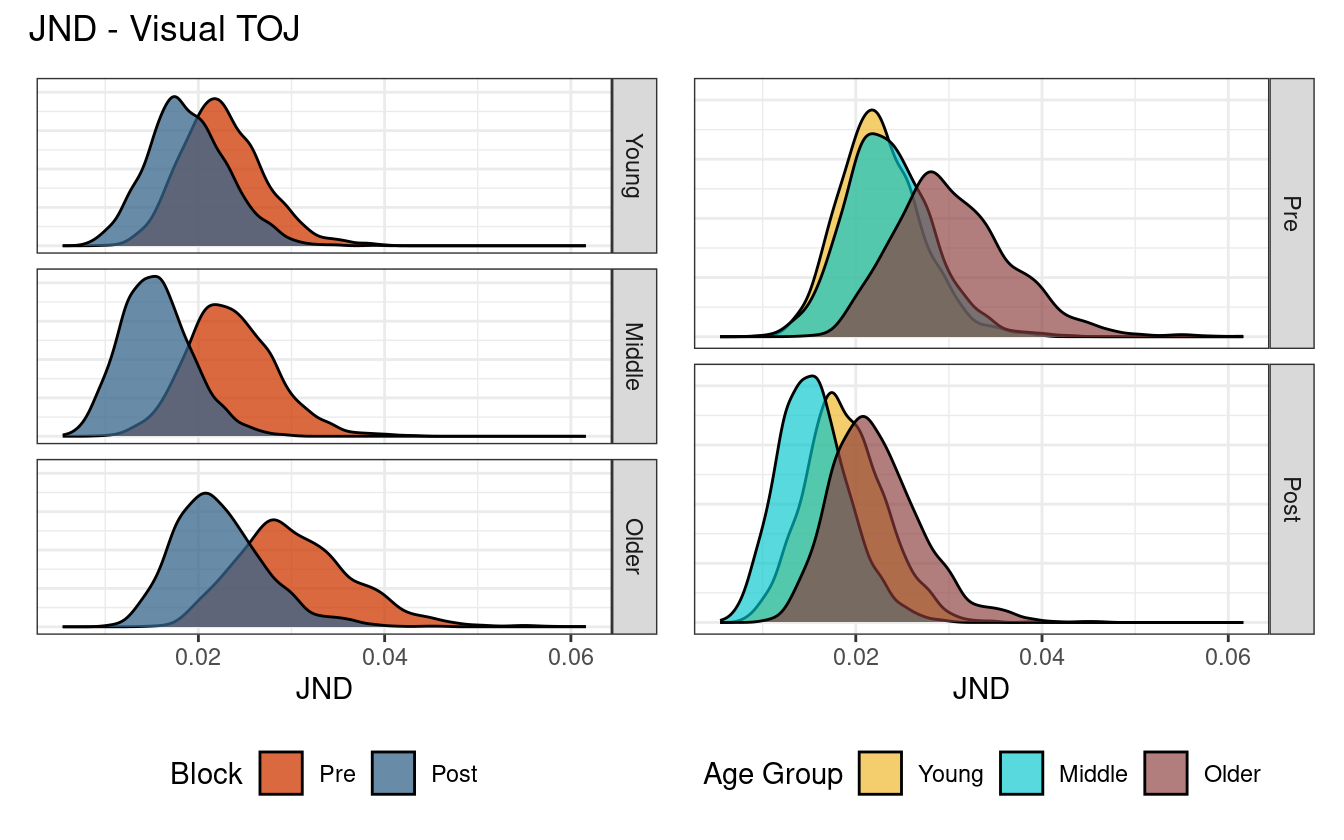
\includegraphics[width=0.85\linewidth]{050-results_files/figure-latex/ch050-Mercury-Rainbow-1} 

}

\caption{Posterior distribution of JND values for the visual task.}\label{fig:ch050-Mercury-Rainbow}
\end{figure}

The story for the visual TOJ task is similar to the audiovisual one - each age group experience heightened temporal sensitivity after recalibration, with the two older age groups receiving more benefit than the younger age group. It's also worth noting that the younger age groups have higher baseline temporal sensitivity, so there may not be as much room for improvement.

\textbf{Duration TOJ Task}

\begin{figure}

{\centering 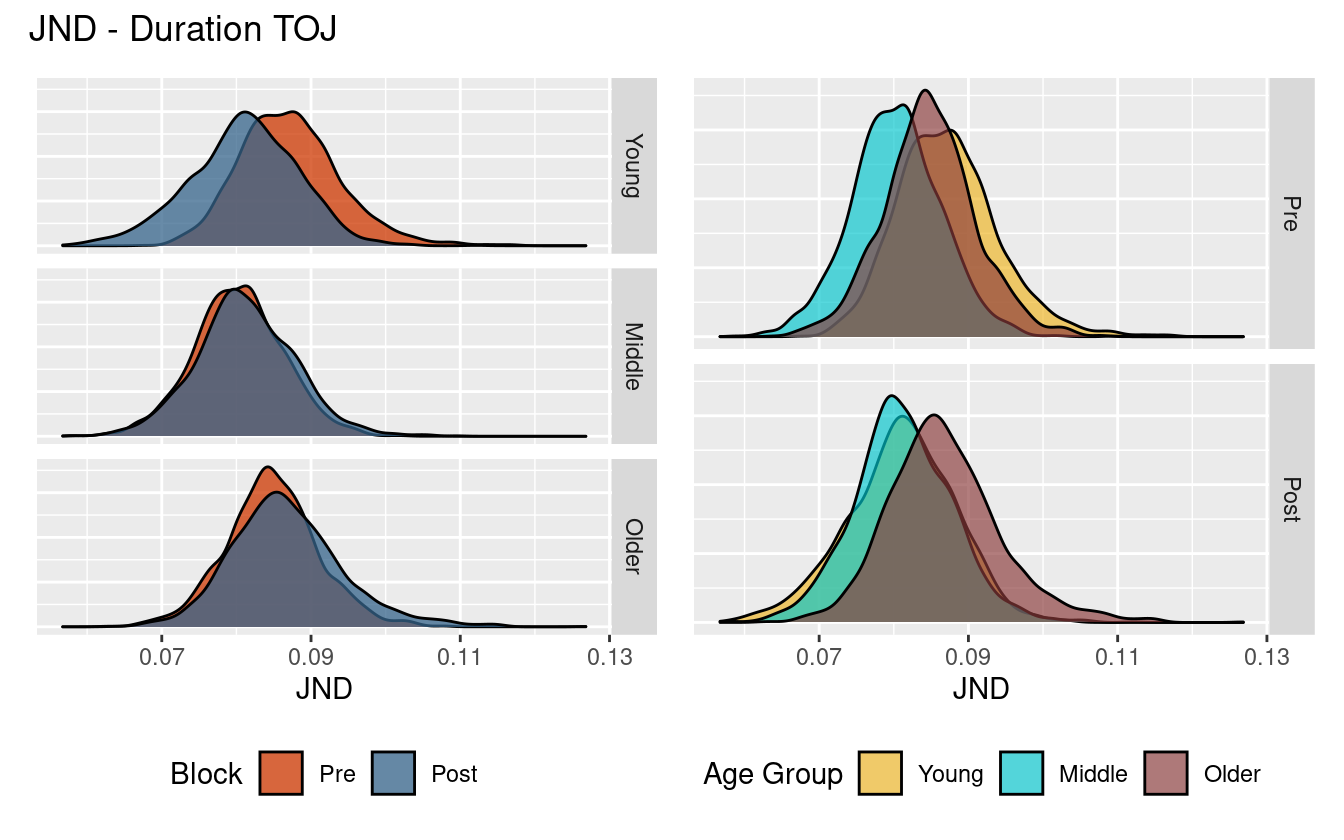
\includegraphics[width=0.85\linewidth]{050-results_files/figure-latex/ch050-Aimless-Planet-1} 

}

\caption{Posterior distribution of JND values for the duration task.}\label{fig:ch050-Aimless-Planet}
\end{figure}

This time the effects of recalibration are not so strong, and just like for the PSS, there is no significant difference between age groups in the duration task.

\textbf{Sensorimotor TOJ Task}

\begin{figure}

{\centering 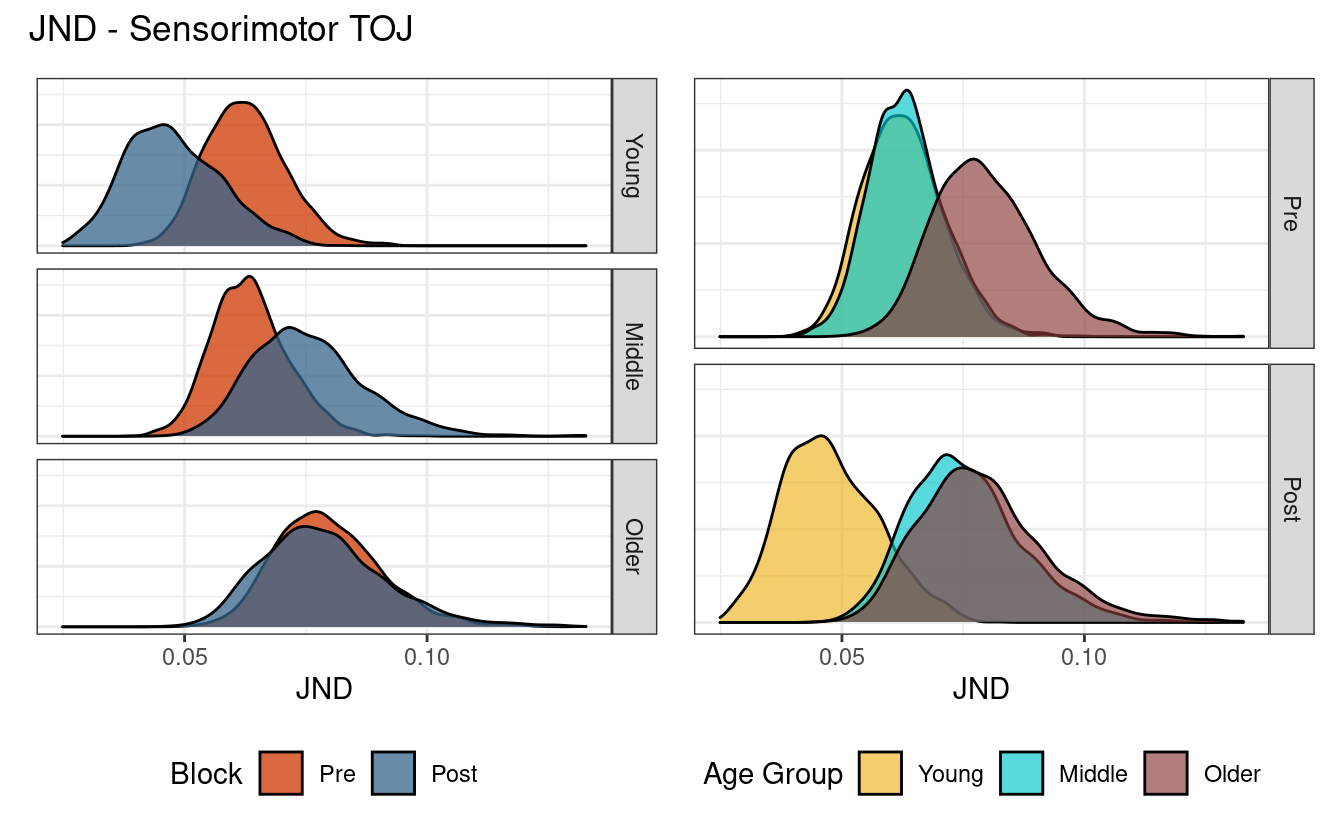
\includegraphics[width=0.85\linewidth]{050-results_files/figure-latex/ch050-Tombstone-Cold-1} 

}

\caption{Posterior distribution of JND values for the sensorimotor task.}\label{fig:ch050-Tombstone-Cold}
\end{figure}

Finally in the sensorimotor task there are mixed results. Temporal recalibration increased the temporal sensitivity in the younger age group, reduced it in the middle age group, and had no effect on the older age group. Clearly the biological factors at play are complex, and the data here is a relatively thin slice of the population. More data and a better calibrated experiment may give better insights into the effects of temporal recalibration.

\hypertarget{lapse-rate-across-age-groups}{%
\section{Lapse Rate across Age Groups}\label{lapse-rate-across-age-groups}}

\begin{figure}

{\centering 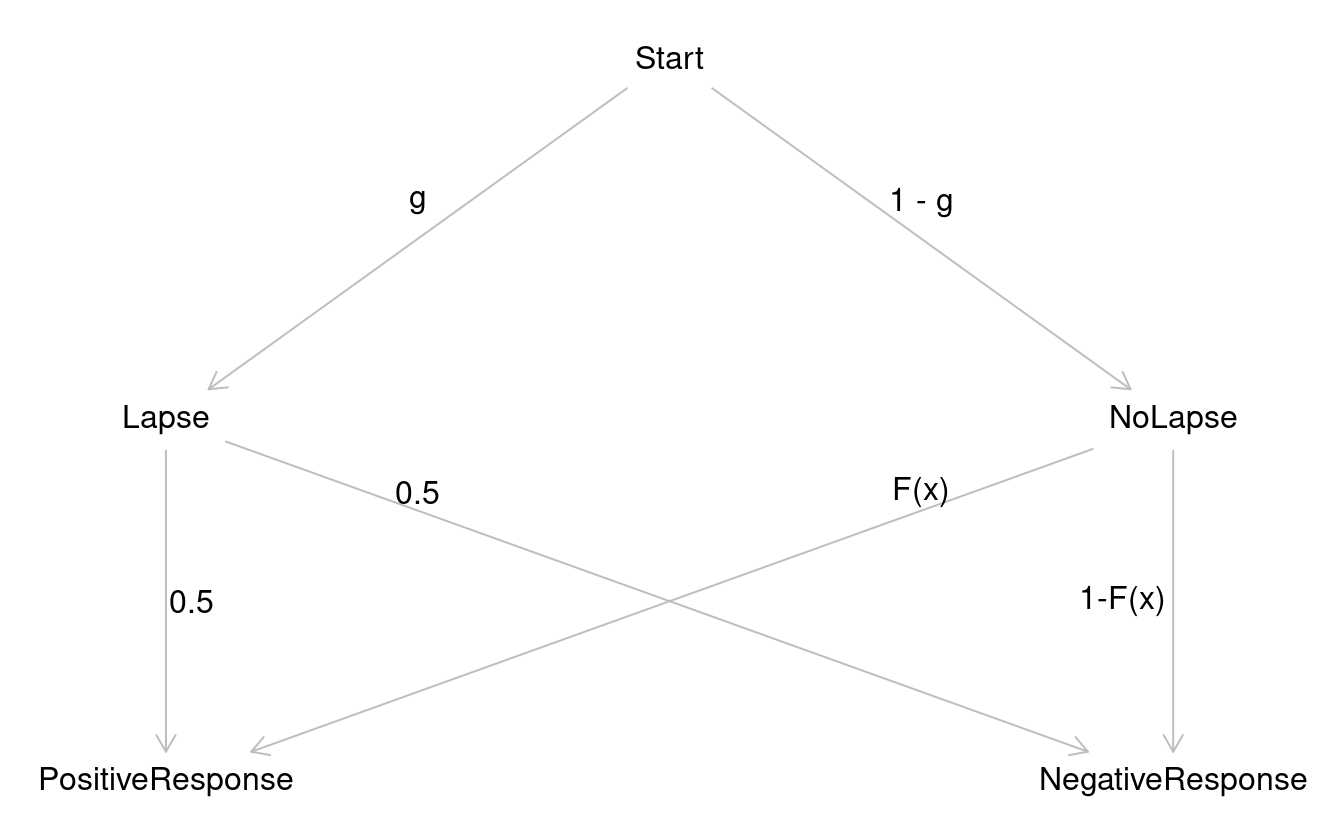
\includegraphics[width=0.85\linewidth]{050-results_files/figure-latex/ch050-Waffle-Hollow-1} 

}

\caption{Process model of the result of a psychometric experiment with the assumption that lapses occur at random and at a fixed rate, and that the subject guesses randomly in the event of a lapse.}\label{fig:ch050-Waffle-Hollow}
\end{figure}

In the above figure, the outcome of one experiment can be represented as a directed acyclic graph (DAG) where at the start of the experiment, the subject either experiences a lapse in judgment with probability \(\gamma\) or they do not experience a lapse in judgment. If there is no lapse, then they will give a positive response with probability \(F(x)\). If there is a lapse in judgment, then it is assumed that they will respond randomly - e.g.~a fifty-fifty chance of a positive response. In this model of an experiment, the probability of a positive response is the sum of the two paths.

\begin{align}
\mathrm{P}(\textrm{positive}) &= 
  \mathrm{P}(\textrm{lapse}) \cdot \mathrm{P}(\textrm{positive} | \textrm{lapse}) \\
  &\quad + \mathrm{P}(\textrm{no lapse}) \cdot \mathrm{P}(\textrm{positive} | \textrm{no lapse}) \\
  &= \frac{1}{2} \gamma + (1 - \gamma) \cdot F(x)
\end{align}

If we then let \(\gamma = 2\lambda\) then the probability of a positive response becomes

\[
\mathrm{P}(\textrm{positive}) = \lambda + (1 - 2\lambda) \cdot F(x)
\]

This is the lapse model described in \eqref{eq:Psi}! But now there is a little bit more insight into what the parameter \(\lambda\) is. If \(\gamma\) is the true lapse rate, then \(\lambda\) is half the lapse rate. This may sound strange at first, but remember that equation \eqref{eq:Psi} was motivated as a lower and upper bound to the psychometric function, and where the bounds are constrained by the same amount. Here the motivation is from a process model, yet the two lines of reasoning arrive at the same model.

Figure \ref{fig:ch050-Magenta-Finger} shows the distribution of lapse rates for each age group across the four separate tasks. There is no visual trend in the ranks of lapse rates, meaning that no single age group definitively experiences a lower lapse rate than the others, though the middle age group comes close to being the winner and the older age group is more likely to be trailing behind. The distribution of lapse rates does reveal something about the tasks themselves.

\begin{figure}

{\centering 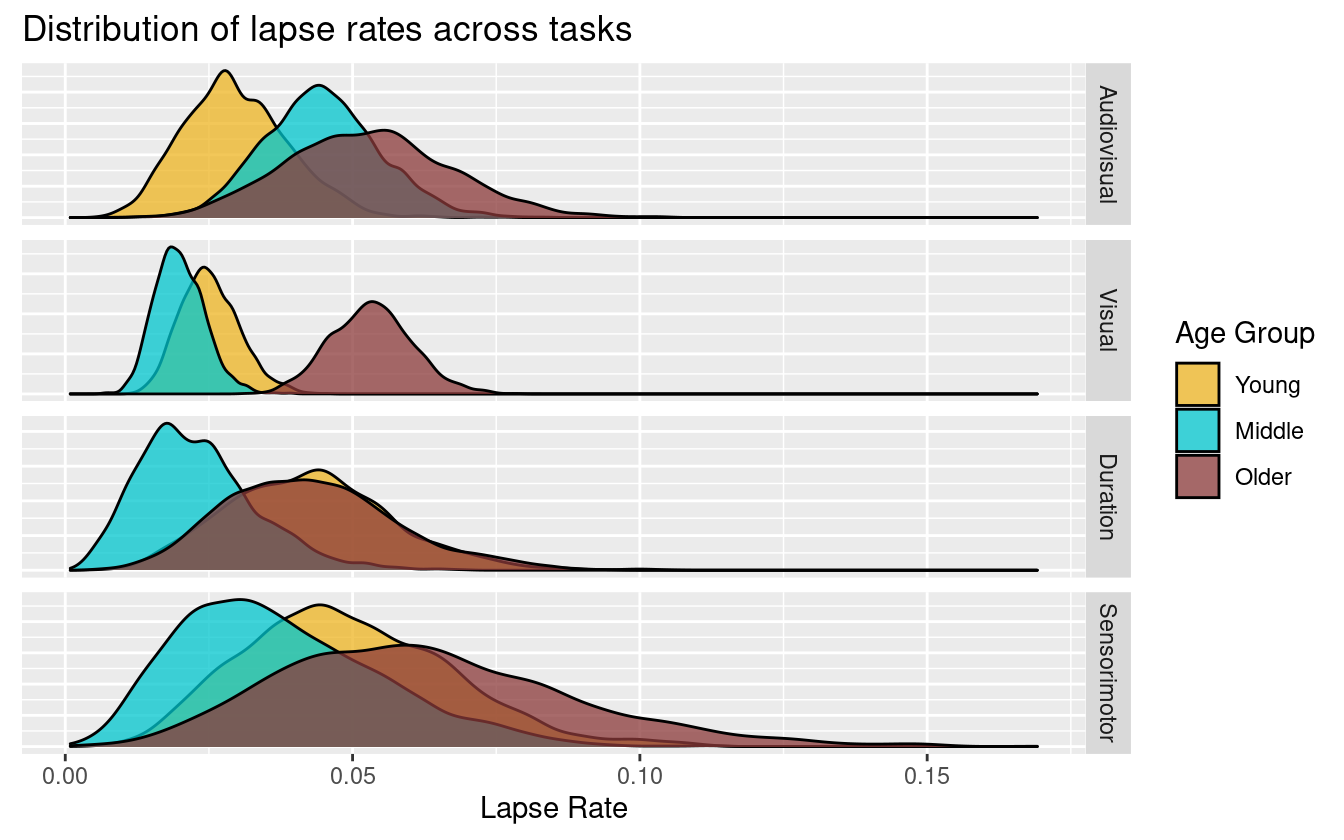
\includegraphics[width=0.85\linewidth]{050-results_files/figure-latex/ch050-Magenta-Finger-1} 

}

\caption{Lapse rates for the different age groups across the four separate tasks. Visually there is no clear trend in lapses by age group, but the concentration of the distributions give insight into the perceived difficulty of a task where more diffuse distributions may indiciate more difficult tasks.}\label{fig:ch050-Magenta-Finger}
\end{figure}

I used the audiovisual data in the first few iterations of building a model and there were no immediate issues, but when I tested the model on the visual data it had trouble expressing the variability at outer SOA values. I noted that one subject had a near perfect response set, and many others had equally impressive performance. The model without a lapse rate was being torn between a very steep slope near the PSS and random variability near the outer SOAs. The remedy was to include a lapse rate (motivated by domain expertise) which allowed for that one extra degree of freedom necessary to reconcile the opposing forces.

Why did the visual data behave this way when the audiovisual data had no issue? That gets deep into the theory of how our brains integrate signals arising from different modalities. Detecting the temporal order of two visual stimuli may be an easier mental task than that of heterogeneous signals. Then consider audiovisual versus duration or sensorimotor. Visual-speech synthesis is a much more common task throughout the day than visual-tactile (sensorimotor), and so perhaps we are better adjusted to such a task as audiovisual. The latent measure of relative performance or task difficulty might be picked up through the lapse rate.

To test this idea, the TOJ experiment could be repeated, and then ask the subject afterwards how they would rate the difficulty of each task. For now, a post-hoc test can be done by comparing the mean and spread of the lapse rates to a \emph{pseuedo difficulty} measure as defined by the mean of the incorrect responses. A response is correct when the sign of the SOA value is concordant with the response, e.g.~a positive SOA and the subject gives the ``positive'' response or a negative SOA and the subject gives the ``negative'' response. Looking at figure \ref{fig:ch050-Magenta-Finger}, I would subjectively rate the tasks from easiest to hardest based on ocular analysis as

\begin{enumerate}
\def\labelenumi{\arabic{enumi}.}
\tightlist
\item
  Visual
\item
  Audiovisual
\item
  Duration
\item
  Sensorimotor
\end{enumerate}

Again, this ranking is based on the mean (lower intrinsically meaning easier) and the spread (less diffuse implying more agreement of difficulty between age groups). The visual task has the tightest distribution of lapse rates, and the sensorimotor has the widest spread, so I can rank those first and last respectively. Audiovisual and duration are very similar in mean and spread, but the audiovisual has a bit more agreement between the young and middle age groups, so second and third go to audiovisual and duration. Table \ref{tab:ch050-Orange-Tigerfish} shows the results arranged by increasing pseudo difficulty. As predicted, the visual task is squarely at the top and the sensorimotor is fully at the bottom. The only out of place group is the audiovisual task for the older age group, which is about equal to the older age group during the duration task. In fact, within tasks, the older age group always comes in last in terms of proportion of correct responses, while the young and middle age groups trade back and forth.

\begin{table}[!h]

\caption{\label{tab:ch050-Orange-Tigerfish}Relative difficulty of the different tasks by age group. The difficulty is measured by the proportion of incorrect responses.}
\centering
\begin{tabular}[t]{l|l|r}
\hline
Task & Age Group & Pseudo Difficulty\\
\hline
visual & Middle Age & 0.03\\
\hline
visual & Young Adult & 0.03\\
\hline
visual & Older Adult & 0.06\\
\hline
audiovisual & Young Adult & 0.12\\
\hline
audiovisual & Middle Age & 0.12\\
\hline
duration & Middle Age & 0.14\\
\hline
duration & Young Adult & 0.16\\
\hline
duration & Older Adult & 0.17\\
\hline
audiovisual & Older Adult & 0.17\\
\hline
sensorimotor & Young Adult & 0.22\\
\hline
sensorimotor & Middle Age & 0.24\\
\hline
sensorimotor & Older Adult & 0.29\\
\hline
\end{tabular}
\end{table}

One way to remove the uncertainty of the lapse rate could be to have some trials with very large SOA values. The reasoning is that if the difficulty of a task (given an SOA value) is lowered, than an incorrect response is more likely to be due to a true lapse in judgment as opposed to a genuinely incorrect response. \citet{wichmann2001b} recommends at least one sample at \(\pi \ge 0.95\) is necessary for reliable bootstrap confidence intervals, so the same reasoning can be applied when using Bayesian credible intervals. For a task such as visual TOJ, the \(90\%\) level may occur at an SOA of \(\approx 40\)ms while for the audiovisual TOJ it may be \(\approx 220\)ms, so the sampling scheme for psychometric experiments must be tuned to the task.

\citet{wichmann2001a} experimentally determined that the lapse rate for trained observers is between \(0\%\) and \(5\%\), and the data in this paper loosely agree with that conclusion. Any excess in lapse rate may be attributed to the perceived task difficulty and a sub-optimal sampling scheme. Since the visual TOJ task is relatively the easiest, the estimated lapse rates are more believable as true lapse rates, and fall closely within the \((0, 0.05)\) range.

\hypertarget{discussion}{%
\chapter{Discussion}\label{discussion}}

\hypertarget{experimental-design}{%
\section{Experimental Design}\label{experimental-design}}

\hypertarget{results-1}{%
\section{Results}\label{results-1}}

\hypertarget{model-comparison-vs.-selection}{%
\section{Model Comparison vs.~Selection}\label{model-comparison-vs.-selection}}

\hypertarget{developing-a-model}{%
\section{Developing a Model}\label{developing-a-model}}

\hypertarget{reproducible-results}{%
\section{Reproducible Results}\label{reproducible-results}}

\hypertarget{conclusion}{%
\chapter{Conclusion}\label{conclusion}}

\begin{itemize}
\tightlist
\item
  Rehash of results
\item
  Point out my direct contributions
\item
  Future work
\item
  Final word
\end{itemize}

\hypertarget{appendix-appendix}{%
\appendix}


\hypertarget{supplementary-code}{%
\chapter{Supplementary Code}\label{supplementary-code}}

\textbf{Eight Schools Model}

\begin{verbatim}
data {
  int<lower=0> J;
  vector[J] y;
  vector<lower=0>[J] sigma;
}
parameters {
  real mu;
  real<lower=0> tau;
  vector[J] theta;
}
model {
  mu ~ normal(0, 10);
  tau ~ cauchy(0, 10);
  theta ~ normal(mu, tau);
  y ~ normal(theta, sigma);
}
\end{verbatim}
%==============================================================================26
\backmatter
%==============================================================================27
\bibliography{bibliography.bib}
%==============================================================================28
% Place here anything that you would like to come
% after the appendix, references, etc
%==============================================================================29
\end{document}
